
\documentclass[main.tex]{subfiles}

\begin{document}
\graphicspath{{imagenes/tema9/}{../imagenes/tema9/}}

\portadatema{9}{Interpolación I}
\begin{frame}[t]{Interpolación: introducción}
La \textbf{interpolación} permite obtener nuevos valores a partir de un conjunto discreto de puntos conocidos.
\bigskip
Para ello se construye una función que pase por esos puntos.
\bigskip
Un problema relacionado es aproximar una función complicada mediante otra más sencilla.
\end{frame}
\begin{frame}[t]{Aplicaciones informáticas}
La interpolación tiene numerosas aplicaciones en informática:
\begin{itemize}
\item Compresión de vídeo.
\item Cambio de frecuencia de muestreo en sonido.
\item Cambio de tamaño de imágenes.
\item Animación de parámetros en realidad virtual.
\end{itemize}
\end{frame}
\begin{frame}[t]{Nodos y función interpolante}
A partir de los puntos conocidos
\[(x_k,y_k),\qquad k=1,\ldots,n,\]
buscamos una función $f$ que cumpla
\[f(x_k)=y_k,\qquad k=1,\ldots,n.\]
Los puntos son los \textbf{nodos} y $f$ es la \textbf{función interpolante}.
\end{frame}
\begin{frame}[t]{Nodos y función interpolante}
\begin{columns}\column{.49\textwidth}\figura{nodos.png}{1}{.65}\column{.49\textwidth}\figura{interpolante.png}{1}{.65}\end{columns}
\end{frame}
\begin{frame}[t]{Elección del interpolante}
La función de interpolación se elige teniendo en cuenta la facilidad de cálculo y el comportamiento de la aproximación.
\end{frame}
\begin{frame}[t]{Interpolación lineal}
La interpolación más sencilla conecta dos puntos mediante una recta.
\medskip
Su precisión depende de la función y de la distancia entre los nodos.\figura{lineal.png}{.8}{.60}
\end{frame}
\begin{frame}[t]{Familias de funciones}
Familias utilizadas para interpolar:
\begin{enumerate}
\item Polinomios.
\item Funciones trigonométricas.
\item Funciones exponenciales.
\item Funciones racionales.
\end{enumerate}
\bigskip
Utilizaremos funciones polinómicas.
\end{frame}
\begin{frame}[t]{Interpolación polinómica}
\small
Dados $n+1$ puntos $(x_0,y_0),\ldots,(x_n,y_n)\in\mathbb{R}^2$, con abscisas distintas dos a dos, buscamos un polinomio de grado $\le n$ tal que
\[P_n(x_i)=y_i,\qquad i=0,\ldots,n.\]
Si los datos provienen de una función $f$, la condición es
\[P_n(x_i)=f(x_i),\qquad i=0,\ldots,n.\]
\end{frame}
\begin{frame}[t]{Aproximación mediante polinomios}
Una interpretación de interpolar es aproximar una función mediante un polinomio que coincida con ella en los nodos.
\bigskip
Antes de estudiar esta construcción, recordamos los polinomios de Taylor.
\end{frame}
\begin{frame}[t]{Polinomios de Taylor}
Para estudiar una función cerca de un punto $a$, podemos sustituirla por una función más sencilla.
\bigskip
Si la función tiene las derivadas necesarias, la aproximamos cerca de $a$ mediante potencias de $x-a$.
\bigskip
Los polinomios de Taylor se construyen con las sucesivas derivadas en $a$.
\end{frame}
\begin{frame}[t]{Taylor y resto}
\small Si $f\in C^{n+1}([a,b])$ y $x_0,x\in[a,b]$, existe $\xi$ entre $x_0$ y $x$ tal que
\[f(x)=P_n(x)+R_n(x,\xi).\]
\begin{columns}\column{.64\textwidth}
\[P_n(x)=\sum_{k=0}^n\frac{f^{(k)}(x_0)}{k!}(x-x_0)^k.\]
\[R_n(x,\xi)=\frac{f^{(n+1)}(\xi)}{(n+1)!}(x-x_0)^{n+1}.\]
\column{.34\textwidth}\figura{taylor.png}{1}{.43}\end{columns}
\end{frame}
\begin{frame}[t]{Polinomio y resto de Taylor}
\small El polinomio de Taylor de orden $n$ es
\begin{align*}
P_n(x)={}&f(x_0)+f'(x_0)(x-x_0)+\frac{f''(x_0)}{2!}(x-x_0)^2\\
&+\cdots+\frac{f^{(n)}(x_0)}{n!}(x-x_0)^n.
\end{align*}
$R_n$ es el \textbf{resto de Taylor} o \textbf{error de truncamiento}.
\medskip
Para $n$ fijo, el resto tiende a cero cuando $x\to x_0$. Para que tienda a cero al aumentar $n$ se necesitan condiciones adicionales.
\end{frame}
\begin{frame}[t]{Aproximaciones sucesivas de Taylor}
\small
Las aproximaciones usan las derivadas de $f$ en $x_0$:
\begin{align*}
P_1(x)&=f(x_0)+f'(x_0)(x-x_0),\\
P_2(x)&=P_1(x)+\frac{f''(x_0)}{2!}(x-x_0)^2,\\
P_3(x)&=P_2(x)+\frac{f^{(3)}(x_0)}{3!}(x-x_0)^3,\\
P_n(x)&=P_{n-1}(x)+\frac{f^{(n)}(x_0)}{n!}(x-x_0)^n.
\end{align*}
En cada caso, $\Delta f(x)=f(x)-P_n(x)=R_n(x,\xi)$.
\end{frame}
\begin{frame}[t]{Error de truncamiento}
El error viene dado por el resto:
\[|f(x)-P_n(x)|=|R_n(x,\xi)|.\]
Si $|f^{(n+1)}(t)|\le M$ entre $x_0$ y $x$, entonces
\[|R_n(x,\xi)|\le\frac{M}{(n+1)!}|x-x_0|^{n+1}.\]
Aumentar el orden puede mejorar la aproximación cerca del centro, pero el error no disminuye necesariamente en cada paso para cualquier función y punto.
\end{frame}
\begin{frame}[t]{Polinomios de Maclaurin}
\small Si $x_0=0$, los polinomios de Taylor se llaman de \textbf{Maclaurin}.
\begin{align*}
P_1(x)&=f(0)+f'(0)x,\\
P_2(x)&=f(0)+f'(0)x+\frac{f''(0)}{2}x^2,\\
P_3(x)&=f(0)+f'(0)x+\frac{f''(0)}{2}x^2+\frac{f^{(3)}(0)}{6}x^3,\\
P_n(x)&=P_{n-1}(x)+\frac{f^{(n)}(0)}{n!}x^n.
\end{align*}
\end{frame}
\begin{frame}[t]{Maclaurin: ejemplo}
Aproximar $\cos(1)$ mediante polinomios de Maclaurin de órdenes 2 y 4.
\end{frame}
\begin{frame}[t]{Maclaurin: construcción}
\small Aproximar $\cos(1)$ con órdenes 2 y 4.
\begin{columns}[T]\column{.63\textwidth}
\[P_2(x)=1-\frac{x^2}{2}.\]
\[P_4(x)=1-\frac{x^2}{2}+\frac{x^4}{24}.\]
\[P_n(x)=\sum_{k=0}^n\frac{f^{(k)}(0)}{k!}x^k.\]
\column{.35\textwidth}
\begin{align*}f(x)&=\cos x,\\f'(x)&=-\sin x,\\f''(x)&=-\cos x,\\f^{(3)}(x)&=\sin x,\\f^{(4)}(x)&=\cos x.\end{align*}
\end{columns}
\end{frame}
\begin{frame}[t]{Maclaurin: evaluación}
\[P_2(x)=1-\frac{x^2}{2},\qquad P_2(1)=\frac12.\]
\[P_4(x)=1-\frac{x^2}{2}+\frac{x^4}{24}.\]
\[\cos(1)\approx P_4(1)=1-\frac12+\frac1{24}=\frac{13}{24}.\]
\end{frame}
\begin{frame}[t]{Maclaurin para el coseno}
\small Polinomios de órdenes 2, 4, 6 y 8 para $\cos x$.\begin{columns}\column{.49\textwidth}\figura{cos2.png}{1}{.30}\figura{cos6.png}{1}{.30}\column{.49\textwidth}\figura{cos4.png}{1}{.30}\figura{cos8.png}{1}{.30}\end{columns}
\end{frame}
\begin{frame}[t]{Existencia y unicidad}
\textbf{Teorema.} Si $x_0,\ldots,x_n$ son reales distintos dos a dos, para cualesquiera valores $y_0,\ldots,y_n$ existe un único polinomio $P_n$ de grado $\le n$ tal que
\[P_n(x_i)=y_i,\qquad i=0,\ldots,n.\]
\bigskip
El teorema garantiza que podemos interpolar cualquier conjunto de datos con abscisas distintas.
\medskip
El problema es construir el polinomio.
\end{frame}
\begin{frame}[t]{Teorema de Weierstrass}
\textbf{Teorema.} Si $f$ es continua en $[a,b]$, para todo $\varepsilon>0$ existe un polinomio $P$ tal que
\[|f(x)-P(x)|<\varepsilon\qquad\text{para todo }x\in[a,b].\]
\bigskip
Toda función continua en un intervalo cerrado y acotado admite una aproximación polinómica uniforme con la precisión deseada.
\medskip
El teorema no impone que $P$ interpole unos nodos prefijados.
\end{frame}
\begin{frame}[t]{Raíces y factores}
Si un polinomio tiene una raíz en $x_i$, contiene el factor $(x-x_i)$.
\medskip
Un polinomio no nulo de grado $n+1$ con raíces distintas $x_0,\ldots,x_n$ tiene la forma
\[P(x)=c(x-x_0)\cdots(x-x_n),\qquad c\ne0.\]\figura{raices.png}{.70}{.40}
\end{frame}
\begin{frame}[t]{Bases de Lagrange}
\small $L_{n,k}$ se anula en todos los nodos salvo $x_k$, donde vale 1.
\[L_{n,k}(x)=\prod_{\substack{j=0\\j\ne k}}^n\frac{x-x_j}{x_k-x_j}.\]\[L_{n,k}(x_j)=\begin{cases}1,&j=k,\\0,&j\ne k.\end{cases}\]\figura{base.png}{.68}{.33}
\end{frame}
\begin{frame}[t]{Polinomio de Lagrange}
El polinomio interpolante de grado $\le n$ es
\[P_n(x)=\sum_{k=0}^n f(x_k)L_{n,k}(x).\]\[P_n(x)=f(x_0)L_{n,0}(x)+\cdots+f(x_n)L_{n,n}(x).\]
Los multiplicadores de Lagrange son
\[L_{n,k}(x)=\prod_{\substack{j=0\\j\ne k}}^n\frac{x-x_j}{x_k-x_j}.\]
\end{frame}
\begin{frame}[t]{Lagrange de grado uno}
\small Conocidos $x_0,x_1$ y $f(x_0),f(x_1)$:
\[L_{1,0}(x)=\frac{x-x_1}{x_0-x_1},\qquad
L_{1,1}(x)=\frac{x-x_0}{x_1-x_0}.\]
\[P_1(x)=f(x_0)L_{1,0}(x)+f(x_1)L_{1,1}(x).\]
\[P_1(x)=f(x_0)\frac{x-x_1}{x_0-x_1}+f(x_1)\frac{x-x_0}{x_1-x_0}.\]
Es una interpolación lineal.
\end{frame}
\begin{frame}[t]{Lagrange de grado dos}
\small Conocidos tres nodos $x_0,x_1,x_2$ y sus valores:\begin{align*}L_{2,0}(x)&=\frac{(x-x_1)(x-x_2)}{(x_0-x_1)(x_0-x_2)},\\L_{2,1}(x)&=\frac{(x-x_0)(x-x_2)}{(x_1-x_0)(x_1-x_2)},\\L_{2,2}(x)&=\frac{(x-x_0)(x-x_1)}{(x_2-x_0)(x_2-x_1)},\\\end{align*}\[P_2(x)=\sum_{k=0}^2f(x_k)L_{2,k}(x).\]
\end{frame}
\begin{frame}[t]{Comparación de grados uno y dos}
\small Cada $L_{2,k}$ incorpora una raíz más que el correspondiente $L_{1,k}$. $P_2$ suma un término más que $P_1$.
\[P_1(x)=f(x_0)\frac{x-x_1}{x_0-x_1}+f(x_1)\frac{x-x_0}{x_1-x_0}.\]
\begin{align*}
P_2(x)={}&f(x_0)\frac{x-x_1}{x_0-x_1}\frac{x-x_2}{x_0-x_2}\\
&+f(x_1)\frac{x-x_0}{x_1-x_0}\frac{x-x_2}{x_1-x_2}\\
&+f(x_2)\frac{(x-x_0)(x-x_1)}{(x_2-x_0)(x_2-x_1)}.
\end{align*}
\end{frame}
\begin{frame}[t]{Lagrange: ejemplo}
\par\noindent\begin{minipage}[t][7.5mm][t]{\textwidth}\small\strut $f(x)=(x/2)^{x-2}$; evaluar en $x=5/2$. Datos: $f(2)=1$, $f(3)=3/2$.\end{minipage}\par\nointerlineskip
\begin{columns}[T]\column{.72\textwidth}\small\setlength{\abovedisplayskip}{4pt}\setlength{\belowdisplayskip}{4pt}\[L_{n,k}(x)=\prod_{\substack{j=0\\j\ne k}}^n\frac{x-x_j}{x_k-x_j}.\]\column{.25\textwidth}\begingroup\small\setlength{\tabcolsep}{3pt}\begin{center}\begin{tabular}{|C{.42\textwidth}|C{.42\textwidth}|}\hline
\rule[-2mm]{0pt}{6mm}$x_i$&$f(x_i)$\\\hline
\rule[-2.5mm]{0pt}{6mm}$x_0=2$&$1$\\\hline
\rule[-2.5mm]{0pt}{6mm}$x_1=3$&$\frac{3}{2}$\\\hline
\rule[-2.5mm]{0pt}{6mm}&\\\hline
\rule[-2.5mm]{0pt}{6mm}&\\\hline
\rule[-2.5mm]{0pt}{6mm}&\\\hline
\end{tabular}\end{center}\endgroup\par
\end{columns}
\end{frame}
\begin{frame}[t]{Lagrange: ejemplo}
\par\noindent\begin{minipage}[t][7.5mm][t]{\textwidth}\small\strut $f(x)=(x/2)^{x-2}$; evaluar en $x=5/2$. Datos: $f(2)=1$, $f(3)=3/2$.\end{minipage}\par\nointerlineskip
\begin{columns}[T]\column{.72\textwidth}\small\setlength{\abovedisplayskip}{4pt}\setlength{\belowdisplayskip}{4pt}\small\[L_{1,0}(x)=\frac{x-3}{2-3}=-(x-3).\]
\[L_{1,1}(x)=\frac{x-2}{3-2}=x-2.\]\[P_n(x)=\sum_{k=0}^n f(x_k)L_{n,k}(x).\]\[L_{n,k}(x)=\prod_{\substack{j=0\\j\ne k}}^n\frac{x-x_j}{x_k-x_j}.\]\column{.25\textwidth}\begingroup\small\setlength{\tabcolsep}{3pt}\begin{center}\begin{tabular}{|C{.42\textwidth}|C{.42\textwidth}|}\hline
\rule[-2mm]{0pt}{6mm}$x_i$&$f(x_i)$\\\hline
\rule[-2.5mm]{0pt}{6mm}$x_0=2$&$1$\\\hline
\rule[-2.5mm]{0pt}{6mm}$x_1=3$&$\frac{3}{2}$\\\hline
\rule[-2.5mm]{0pt}{6mm}&\\\hline
\rule[-2.5mm]{0pt}{6mm}&\\\hline
\rule[-2.5mm]{0pt}{6mm}&\\\hline
\end{tabular}\end{center}\endgroup\par
\end{columns}
\end{frame}
\begin{frame}[t]{Lagrange: ejemplo}
\par\noindent\begin{minipage}[t][7.5mm][t]{\textwidth}\small\strut $f(x)=(x/2)^{x-2}$; evaluar en $x=5/2$. Datos: $f(2)=1$, $f(3)=3/2$.\end{minipage}\par\nointerlineskip
\begin{columns}[T]\column{.72\textwidth}\small\setlength{\abovedisplayskip}{4pt}\setlength{\belowdisplayskip}{4pt}\small\[L_{1,0}(x)=\frac{x-3}{2-3}=-(x-3).\]
\[L_{1,1}(x)=\frac{x-2}{3-2}=x-2.\]\[P_1(x)=-(x-3)+\frac32(x-2)=\frac{x}{2}.\]
\[P_1(5/2)=\frac54=1.25.\]\column{.25\textwidth}\begingroup\small\setlength{\tabcolsep}{3pt}\begin{center}\begin{tabular}{|C{.42\textwidth}|C{.42\textwidth}|}\hline
\rule[-2mm]{0pt}{6mm}$x_i$&$f(x_i)$\\\hline
\rule[-2.5mm]{0pt}{6mm}$x_0=2$&$1$\\\hline
\rule[-2.5mm]{0pt}{6mm}$x_1=3$&$\frac{3}{2}$\\\hline
\rule[-2.5mm]{0pt}{6mm}&\\\hline
\rule[-2.5mm]{0pt}{6mm}&\\\hline
\rule[-2.5mm]{0pt}{6mm}&\\\hline
\end{tabular}\end{center}\endgroup\par
\end{columns}
\end{frame}
\begin{frame}[t]{Lagrange: ejemplo}
\par\noindent\begin{minipage}[t][7.5mm][t]{\textwidth}\small\strut $f(x)=(x/2)^{x-2}$; evaluar en $x=5/2$. Datos: $f(2)=1$, $f(3)=3/2$.\end{minipage}\par\nointerlineskip
\begin{columns}[T]\column{.72\textwidth}\small\setlength{\abovedisplayskip}{4pt}\setlength{\belowdisplayskip}{4pt}\[f(5/2)=\left(\frac54\right)^{1/2}=\frac{\sqrt5}{2}\approx1.118034.\]\[P_1(x)=-(x-3)+\frac32(x-2)=\frac{x}{2}.\]
\[P_1(5/2)=\frac54=1.25.\]\column{.25\textwidth}\begingroup\small\setlength{\tabcolsep}{3pt}\begin{center}\begin{tabular}{|C{.42\textwidth}|C{.42\textwidth}|}\hline
\rule[-2mm]{0pt}{6mm}$x_i$&$f(x_i)$\\\hline
\rule[-2.5mm]{0pt}{6mm}$x_0=2$&$1$\\\hline
\rule[-2.5mm]{0pt}{6mm}$x_1=3$&$\frac{3}{2}$\\\hline
\rule[-2.5mm]{0pt}{6mm}&\\\hline
\rule[-2.5mm]{0pt}{6mm}&\\\hline
\rule[-2.5mm]{0pt}{6mm}&\\\hline
\end{tabular}\end{center}\endgroup\par
\end{columns}
\end{frame}
\begin{frame}[t]{Lagrange: ejemplo}
\par\noindent\begin{minipage}[t][7.5mm][t]{\textwidth}\small\strut $f(x)=(x/2)^{x-2}$; evaluar en $x=5/2$. Datos: $f(2)=1$, $f(3)=3/2$.\end{minipage}\par\nointerlineskip
\begin{columns}[T]\column{.72\textwidth}\small\setlength{\abovedisplayskip}{4pt}\setlength{\belowdisplayskip}{4pt}\figura{grado1.png}{1}{.43}\[f(5/2)=\left(\frac54\right)^{1/2}=\frac{\sqrt5}{2}\approx1.118034.\]\[P_1(5/2)=1.25,\qquad |f(5/2)-P_1(5/2)|\approx0.131966.\]\column{.25\textwidth}\begingroup\small\setlength{\tabcolsep}{3pt}\begin{center}\begin{tabular}{|C{.42\textwidth}|C{.42\textwidth}|}\hline
\rule[-2mm]{0pt}{6mm}$x_i$&$f(x_i)$\\\hline
\rule[-2.5mm]{0pt}{6mm}$x_0=2$&$1$\\\hline
\rule[-2.5mm]{0pt}{6mm}$x_1=3$&$\frac{3}{2}$\\\hline
\rule[-2.5mm]{0pt}{6mm}&\\\hline
\rule[-2.5mm]{0pt}{6mm}&\\\hline
\rule[-2.5mm]{0pt}{6mm}&\\\hline
\end{tabular}\end{center}\endgroup\par
\end{columns}
\end{frame}
\begin{frame}[t]{Lagrange: ejemplo}
\par\noindent\begin{minipage}[t][7.5mm][t]{\textwidth}\small\strut $f(x)=(x/2)^{x-2}$; evaluar en $x=5/2$. Nodos: $1,\ldots,3$. Polinomio de grado $\le 2$.\end{minipage}\par\nointerlineskip
\begin{columns}[T]\column{.72\textwidth}\small\setlength{\abovedisplayskip}{4pt}\setlength{\belowdisplayskip}{4pt}\[L_{n,k}(x)=\prod_{\substack{j=0\\j\ne k}}^n\frac{x-x_j}{x_k-x_j}.\]\column{.25\textwidth}\begingroup\small\setlength{\tabcolsep}{3pt}\begin{center}\begin{tabular}{|C{.42\textwidth}|C{.42\textwidth}|}\hline
\rule[-2mm]{0pt}{6mm}$x_i$&$f(x_i)$\\\hline
\rule[-2.5mm]{0pt}{6mm}$x_0=1$&$2$\\\hline
\rule[-2.5mm]{0pt}{6mm}$x_1=2$&$1$\\\hline
\rule[-2.5mm]{0pt}{6mm}$x_2=3$&$\frac{3}{2}$\\\hline
\rule[-2.5mm]{0pt}{6mm}&\\\hline
\rule[-2.5mm]{0pt}{6mm}&\\\hline
\end{tabular}\end{center}\endgroup\par
\end{columns}
\end{frame}
\begin{frame}[t]{Lagrange: ejemplo}
\par\noindent\begin{minipage}[t][7.5mm][t]{\textwidth}\small\strut $f(x)=(x/2)^{x-2}$; evaluar en $x=5/2$. Nodos: $1,\ldots,3$. Polinomio de grado $\le 2$.\end{minipage}\par\nointerlineskip
\begin{columns}[T]\column{.72\textwidth}\small\setlength{\abovedisplayskip}{4pt}\setlength{\belowdisplayskip}{4pt}\scriptsize\begin{align*}L_{2,0}(x)&=\frac{(x-2)(x-3)}{(1-2)(1-3)},\\L_{2,1}(x)&=\frac{(x-1)(x-3)}{(2-1)(2-3)},\\L_{2,2}(x)&=\frac{(x-1)(x-2)}{(3-1)(3-2)},\\\end{align*}\column{.25\textwidth}\begingroup\small\setlength{\tabcolsep}{3pt}\begin{center}\begin{tabular}{|C{.42\textwidth}|C{.42\textwidth}|}\hline
\rule[-2mm]{0pt}{6mm}$x_i$&$f(x_i)$\\\hline
\rule[-2.5mm]{0pt}{6mm}$x_0=1$&$2$\\\hline
\rule[-2.5mm]{0pt}{6mm}$x_1=2$&$1$\\\hline
\rule[-2.5mm]{0pt}{6mm}$x_2=3$&$\frac{3}{2}$\\\hline
\rule[-2.5mm]{0pt}{6mm}&\\\hline
\rule[-2.5mm]{0pt}{6mm}&\\\hline
\end{tabular}\end{center}\endgroup\par
\end{columns}
\end{frame}
\begin{frame}[t]{Lagrange: ejemplo}
\par\noindent\begin{minipage}[t][7.5mm][t]{\textwidth}\small\strut $f(x)=(x/2)^{x-2}$; evaluar en $x=5/2$. Nodos: $1,\ldots,3$. Polinomio de grado $\le 2$.\end{minipage}\par\nointerlineskip
\begin{columns}[T]\column{.72\textwidth}\small\setlength{\abovedisplayskip}{4pt}\setlength{\belowdisplayskip}{4pt}\scriptsize\begin{align*}L_{2,0}(x)&=\frac{(x-2)(x-3)}{(1-2)(1-3)},\\L_{2,1}(x)&=\frac{(x-1)(x-3)}{(2-1)(2-3)},\\L_{2,2}(x)&=\frac{(x-1)(x-2)}{(3-1)(3-2)},\\\end{align*}\[P_2(x)=\sum_{k=0}^2f(x_k)L_{2,k}(x).\]\column{.25\textwidth}\begingroup\small\setlength{\tabcolsep}{3pt}\begin{center}\begin{tabular}{|C{.42\textwidth}|C{.42\textwidth}|}\hline
\rule[-2mm]{0pt}{6mm}$x_i$&$f(x_i)$\\\hline
\rule[-2.5mm]{0pt}{6mm}$x_0=1$&$2$\\\hline
\rule[-2.5mm]{0pt}{6mm}$x_1=2$&$1$\\\hline
\rule[-2.5mm]{0pt}{6mm}$x_2=3$&$\frac{3}{2}$\\\hline
\rule[-2.5mm]{0pt}{6mm}&\\\hline
\rule[-2.5mm]{0pt}{6mm}&\\\hline
\end{tabular}\end{center}\endgroup\par
\end{columns}
\end{frame}
\begin{frame}[t]{Lagrange: ejemplo}
\par\noindent\begin{minipage}[t][7.5mm][t]{\textwidth}\small\strut $f(x)=(x/2)^{x-2}$; evaluar en $x=5/2$. Nodos: $1,\ldots,3$. Polinomio de grado $\le 2$.\end{minipage}\par\nointerlineskip
\begin{columns}[T]\column{.72\textwidth}\small\setlength{\abovedisplayskip}{4pt}\setlength{\belowdisplayskip}{4pt}\small\begin{align*}
P_2(x)={}&2\frac{(x-2)(x-3)}{2}\\
&-\frac{(x-1)(x-3)}{1}\\
&+\frac32\frac{(x-1)(x-2)}{2}.
\end{align*}\[P_n(x)=\sum_{k=0}^n f(x_k)L_{n,k}(x).\]\column{.25\textwidth}\begingroup\small\setlength{\tabcolsep}{3pt}\begin{center}\begin{tabular}{|C{.42\textwidth}|C{.42\textwidth}|}\hline
\rule[-2mm]{0pt}{6mm}$x_i$&$f(x_i)$\\\hline
\rule[-2.5mm]{0pt}{6mm}$x_0=1$&$2$\\\hline
\rule[-2.5mm]{0pt}{6mm}$x_1=2$&$1$\\\hline
\rule[-2.5mm]{0pt}{6mm}$x_2=3$&$\frac{3}{2}$\\\hline
\rule[-2.5mm]{0pt}{6mm}&\\\hline
\rule[-2.5mm]{0pt}{6mm}&\\\hline
\end{tabular}\end{center}\endgroup\par
\end{columns}
\end{frame}
\begin{frame}[t]{Lagrange: ejemplo}
\par\noindent\begin{minipage}[t][7.5mm][t]{\textwidth}\small\strut $f(x)=(x/2)^{x-2}$; evaluar en $x=5/2$. Nodos: $1,\ldots,3$. Polinomio de grado $\le 2$.\end{minipage}\par\nointerlineskip
\begin{columns}[T]\column{.72\textwidth}\small\setlength{\abovedisplayskip}{4pt}\setlength{\belowdisplayskip}{4pt}\small\begin{align*}
P_2(x)={}&2\frac{(x-2)(x-3)}{2}\\
&-\frac{(x-1)(x-3)}{1}\\
&+\frac32\frac{(x-1)(x-2)}{2}.
\end{align*}\[P_2(5/2)=-\frac14+\frac34+\frac9{16}=\frac{17}{16}=1.0625.\]\column{.25\textwidth}\begingroup\small\setlength{\tabcolsep}{3pt}\begin{center}\begin{tabular}{|C{.42\textwidth}|C{.42\textwidth}|}\hline
\rule[-2mm]{0pt}{6mm}$x_i$&$f(x_i)$\\\hline
\rule[-2.5mm]{0pt}{6mm}$x_0=1$&$2$\\\hline
\rule[-2.5mm]{0pt}{6mm}$x_1=2$&$1$\\\hline
\rule[-2.5mm]{0pt}{6mm}$x_2=3$&$\frac{3}{2}$\\\hline
\rule[-2.5mm]{0pt}{6mm}&\\\hline
\rule[-2.5mm]{0pt}{6mm}&\\\hline
\end{tabular}\end{center}\endgroup\par
\end{columns}
\end{frame}
\begin{frame}[t]{Lagrange: ejemplo}
\par\noindent\begin{minipage}[t][7.5mm][t]{\textwidth}\small\strut $f(x)=(x/2)^{x-2}$; evaluar en $x=5/2$. Nodos: $1,\ldots,3$. Polinomio de grado $\le 2$.\end{minipage}\par\nointerlineskip
\begin{columns}[T]\column{.72\textwidth}\small\setlength{\abovedisplayskip}{4pt}\setlength{\belowdisplayskip}{4pt}\figura{grado2.png}{1}{.29}\[f(5/2)=\left(\frac54\right)^{1/2}=\frac{\sqrt5}{2}\approx1.118034.\]\[P_2(5/2)=-\frac14+\frac34+\frac9{16}=\frac{17}{16}=1.0625.\]\small Error absoluto: $0.055534$.\column{.25\textwidth}\begingroup\small\setlength{\tabcolsep}{3pt}\begin{center}\begin{tabular}{|C{.42\textwidth}|C{.42\textwidth}|}\hline
\rule[-2mm]{0pt}{6mm}$x_i$&$f(x_i)$\\\hline
\rule[-2.5mm]{0pt}{6mm}$x_0=1$&$2$\\\hline
\rule[-2.5mm]{0pt}{6mm}$x_1=2$&$1$\\\hline
\rule[-2.5mm]{0pt}{6mm}$x_2=3$&$\frac{3}{2}$\\\hline
\rule[-2.5mm]{0pt}{6mm}&\\\hline
\rule[-2.5mm]{0pt}{6mm}&\\\hline
\end{tabular}\end{center}\endgroup\par
\end{columns}
\end{frame}
\begin{frame}[t]{Lagrange: ejemplo}
\par\noindent\begin{minipage}[t][7.5mm][t]{\textwidth}\small\strut $f(x)=(x/2)^{x-2}$; evaluar en $x=5/2$. Nodos: $1,\ldots,4$. Polinomio de grado $\le 3$.\end{minipage}\par\nointerlineskip
\begin{columns}[T]\column{.72\textwidth}\small\setlength{\abovedisplayskip}{4pt}\setlength{\belowdisplayskip}{4pt}\[L_{n,k}(x)=\prod_{\substack{j=0\\j\ne k}}^n\frac{x-x_j}{x_k-x_j}.\]\column{.25\textwidth}\begingroup\small\setlength{\tabcolsep}{3pt}\begin{center}\begin{tabular}{|C{.42\textwidth}|C{.42\textwidth}|}\hline
\rule[-2mm]{0pt}{6mm}$x_i$&$f(x_i)$\\\hline
\rule[-2.5mm]{0pt}{6mm}$x_0=1$&$2$\\\hline
\rule[-2.5mm]{0pt}{6mm}$x_1=2$&$1$\\\hline
\rule[-2.5mm]{0pt}{6mm}$x_2=3$&$\frac{3}{2}$\\\hline
\rule[-2.5mm]{0pt}{6mm}$x_3=4$&$4$\\\hline
\rule[-2.5mm]{0pt}{6mm}&\\\hline
\end{tabular}\end{center}\endgroup\par
\end{columns}
\end{frame}
\begin{frame}[t]{Lagrange: ejemplo}
\par\noindent\begin{minipage}[t][7.5mm][t]{\textwidth}\small\strut $f(x)=(x/2)^{x-2}$; evaluar en $x=5/2$. Nodos: $1,\ldots,4$. Polinomio de grado $\le 3$.\end{minipage}\par\nointerlineskip
\begin{columns}[T]\column{.72\textwidth}\small\setlength{\abovedisplayskip}{4pt}\setlength{\belowdisplayskip}{4pt}\scriptsize\begin{align*}L_{3,0}(x)&=\frac{(x-2)(x-3)(x-4)}{(1-2)(1-3)(1-4)},\\L_{3,1}(x)&=\frac{(x-1)(x-3)(x-4)}{(2-1)(2-3)(2-4)},\\L_{3,2}(x)&=\frac{(x-1)(x-2)(x-4)}{(3-1)(3-2)(3-4)},\\L_{3,3}(x)&=\frac{(x-1)(x-2)(x-3)}{(4-1)(4-2)(4-3)},\\\end{align*}\column{.25\textwidth}\begingroup\small\setlength{\tabcolsep}{3pt}\begin{center}\begin{tabular}{|C{.42\textwidth}|C{.42\textwidth}|}\hline
\rule[-2mm]{0pt}{6mm}$x_i$&$f(x_i)$\\\hline
\rule[-2.5mm]{0pt}{6mm}$x_0=1$&$2$\\\hline
\rule[-2.5mm]{0pt}{6mm}$x_1=2$&$1$\\\hline
\rule[-2.5mm]{0pt}{6mm}$x_2=3$&$\frac{3}{2}$\\\hline
\rule[-2.5mm]{0pt}{6mm}$x_3=4$&$4$\\\hline
\rule[-2.5mm]{0pt}{6mm}&\\\hline
\end{tabular}\end{center}\endgroup\par
\end{columns}
\end{frame}
\begin{frame}[t]{Lagrange: ejemplo}
\par\noindent\begin{minipage}[t][7.5mm][t]{\textwidth}\small\strut $f(x)=(x/2)^{x-2}$; evaluar en $x=5/2$. Nodos: $1,\ldots,4$. Polinomio de grado $\le 3$.\end{minipage}\par\nointerlineskip
\begin{columns}[T]\column{.72\textwidth}\small\setlength{\abovedisplayskip}{4pt}\setlength{\belowdisplayskip}{4pt}\scriptsize\begin{align*}L_{3,0}(x)&=\frac{(x-2)(x-3)(x-4)}{(1-2)(1-3)(1-4)},\\L_{3,1}(x)&=\frac{(x-1)(x-3)(x-4)}{(2-1)(2-3)(2-4)},\\L_{3,2}(x)&=\frac{(x-1)(x-2)(x-4)}{(3-1)(3-2)(3-4)},\\L_{3,3}(x)&=\frac{(x-1)(x-2)(x-3)}{(4-1)(4-2)(4-3)},\\\end{align*}\small Para evaluar en un punto, podemos organizar los cálculos en una tabla.\column{.25\textwidth}\begingroup\small\setlength{\tabcolsep}{3pt}\begin{center}\begin{tabular}{|C{.42\textwidth}|C{.42\textwidth}|}\hline
\rule[-2mm]{0pt}{6mm}$x_i$&$f(x_i)$\\\hline
\rule[-2.5mm]{0pt}{6mm}$x_0=1$&$2$\\\hline
\rule[-2.5mm]{0pt}{6mm}$x_1=2$&$1$\\\hline
\rule[-2.5mm]{0pt}{6mm}$x_2=3$&$\frac{3}{2}$\\\hline
\rule[-2.5mm]{0pt}{6mm}$x_3=4$&$4$\\\hline
\rule[-2.5mm]{0pt}{6mm}&\\\hline
\end{tabular}\end{center}\endgroup\par
\end{columns}
\end{frame}
\begin{frame}[t]{Lagrange: tabla de grado tres}
\par\noindent\begin{minipage}[t][12mm][t]{\textwidth}\small\strut $f(x)=(x/2)^{x-2}$; nodos $1,2,3,4$; evaluar en $5/2$.\end{minipage}\par\nointerlineskip
\begingroup\scriptsize\setlength{\tabcolsep}{3pt}\begin{center}\begin{tabular}{|C{.06\textwidth}|C{.10\textwidth}|C{.48\textwidth}|C{.20\textwidth}|}\hline
\rule[-2mm]{0pt}{6mm}$x_i$&$f(x_i)$&$L_{3,i}(x)$&$f(x_i)L_{3,i}(5/2)$\\\hline
\rule[-2.5mm]{0pt}{7mm}$1$&$2$&$\frac{(x-2)(x-3)(x-4)}{-6}$&\\\hline
\rule[-2.5mm]{0pt}{7mm}$2$&$1$&$\frac{(x-1)(x-3)(x-4)}{2}$&\\\hline
\rule[-2.5mm]{0pt}{7mm}$3$&$\frac{3}{2}$&$\frac{(x-1)(x-2)(x-4)}{-2}$&\\\hline
\rule[-2.5mm]{0pt}{7mm}$4$&$4$&$\frac{(x-1)(x-2)(x-3)}{6}$&\\\hline
\rule[-2.5mm]{0pt}{7mm}&&&\\\hline
\end{tabular}\end{center}\endgroup\par
\[P_3(x)=\sum_{i=0}^3 f(x_i)L_{3,i}(x).\]
\end{frame}
\begin{frame}[t]{Lagrange: tabla de grado tres}
\par\noindent\begin{minipage}[t][12mm][t]{\textwidth}\small\strut $f(x)=(x/2)^{x-2}$; nodos $1,2,3,4$; evaluar en $5/2$.\end{minipage}\par\nointerlineskip
\begingroup\scriptsize\setlength{\tabcolsep}{3pt}\begin{center}\begin{tabular}{|C{.06\textwidth}|C{.10\textwidth}|C{.48\textwidth}|C{.20\textwidth}|}\hline
\rule[-2mm]{0pt}{6mm}$x_i$&$f(x_i)$&$L_{3,i}(x)$&$f(x_i)L_{3,i}(5/2)$\\\hline
\rule[-2.5mm]{0pt}{7mm}$1$&$2$&$\frac{(x-2)(x-3)(x-4)}{-6}$&$-\frac{1}{8}$\\\hline
\rule[-2.5mm]{0pt}{7mm}$2$&$1$&$\frac{(x-1)(x-3)(x-4)}{2}$&$\frac{9}{16}$\\\hline
\rule[-2.5mm]{0pt}{7mm}$3$&$\frac{3}{2}$&$\frac{(x-1)(x-2)(x-4)}{-2}$&$\frac{27}{32}$\\\hline
\rule[-2.5mm]{0pt}{7mm}$4$&$4$&$\frac{(x-1)(x-2)(x-3)}{6}$&$-\frac{1}{4}$\\\hline
\rule[-2.5mm]{0pt}{7mm}&&&\\\hline
\end{tabular}\end{center}\endgroup\par
\[P_3(5/2)=-\frac18+\frac9{16}+\frac{27}{32}-\frac14=\frac{33}{32}.\]
\end{frame}
\begin{frame}[t]{Lagrange: ejemplo}
\par\noindent\begin{minipage}[t][7.5mm][t]{\textwidth}\small\strut $f(x)=(x/2)^{x-2}$; evaluar en $x=5/2$. Nodos: $1,\ldots,4$. Polinomio de grado $\le 3$.\end{minipage}\par\nointerlineskip
\begin{columns}[T]\column{.72\textwidth}\small\setlength{\abovedisplayskip}{4pt}\setlength{\belowdisplayskip}{4pt}\figura{grado3.png}{1}{.29}\[f(5/2)=\left(\frac54\right)^{1/2}=\frac{\sqrt5}{2}\approx1.118034.\]\[P_3(5/2)=\frac{33}{32}=1.03125.\]\small Error absoluto: $0.086784$.\column{.25\textwidth}\begingroup\small\setlength{\tabcolsep}{3pt}\begin{center}\begin{tabular}{|C{.42\textwidth}|C{.42\textwidth}|}\hline
\rule[-2mm]{0pt}{6mm}$x_i$&$f(x_i)$\\\hline
\rule[-2.5mm]{0pt}{6mm}$x_0=1$&$2$\\\hline
\rule[-2.5mm]{0pt}{6mm}$x_1=2$&$1$\\\hline
\rule[-2.5mm]{0pt}{6mm}$x_2=3$&$\frac{3}{2}$\\\hline
\rule[-2.5mm]{0pt}{6mm}$x_3=4$&$4$\\\hline
\rule[-2.5mm]{0pt}{6mm}&\\\hline
\end{tabular}\end{center}\endgroup\par
\end{columns}
\end{frame}
\begin{frame}[t]{Lagrange: ejemplo}
\par\noindent\begin{minipage}[t][7.5mm][t]{\textwidth}\small\strut $f(x)=(x/2)^{x-2}$; evaluar en $x=5/2$. Nodos: $1,\ldots,5$. Polinomio de grado $\le 4$.\end{minipage}\par\nointerlineskip
\begin{columns}[T]\column{.72\textwidth}\small\setlength{\abovedisplayskip}{4pt}\setlength{\belowdisplayskip}{4pt}\figura{grado4.png}{1}{.49}\small\[P_4(5/2)=-\frac{15}{192}+\frac{15}{32}+\frac{135}{128}-\frac58+\frac{375}{1024}.\]\column{.25\textwidth}\begingroup\small\setlength{\tabcolsep}{3pt}\begin{center}\begin{tabular}{|C{.42\textwidth}|C{.42\textwidth}|}\hline
\rule[-2mm]{0pt}{6mm}$x_i$&$f(x_i)$\\\hline
\rule[-2.5mm]{0pt}{6mm}$x_0=1$&$2$\\\hline
\rule[-2.5mm]{0pt}{6mm}$x_1=2$&$1$\\\hline
\rule[-2.5mm]{0pt}{6mm}$x_2=3$&$\frac{3}{2}$\\\hline
\rule[-2.5mm]{0pt}{6mm}$x_3=4$&$4$\\\hline
\rule[-2.5mm]{0pt}{6mm}$x_4=5$&$\frac{125}{8}$\\\hline
\end{tabular}\end{center}\endgroup\par
\end{columns}
\end{frame}
\begin{frame}[t]{Lagrange: ejemplo}
\par\noindent\begin{minipage}[t][7.5mm][t]{\textwidth}\small\strut $f(x)=(x/2)^{x-2}$; evaluar en $x=5/2$. Nodos: $1,\ldots,5$. Polinomio de grado $\le 4$.\end{minipage}\par\nointerlineskip
\begin{columns}[T]\column{.72\textwidth}\small\setlength{\abovedisplayskip}{4pt}\setlength{\belowdisplayskip}{4pt}\[L_{n,k}(x)=\prod_{\substack{j=0\\j\ne k}}^n\frac{x-x_j}{x_k-x_j}.\]\column{.25\textwidth}\begingroup\small\setlength{\tabcolsep}{3pt}\begin{center}\begin{tabular}{|C{.42\textwidth}|C{.42\textwidth}|}\hline
\rule[-2mm]{0pt}{6mm}$x_i$&$f(x_i)$\\\hline
\rule[-2.5mm]{0pt}{6mm}$x_0=1$&$2$\\\hline
\rule[-2.5mm]{0pt}{6mm}$x_1=2$&$1$\\\hline
\rule[-2.5mm]{0pt}{6mm}$x_2=3$&$\frac{3}{2}$\\\hline
\rule[-2.5mm]{0pt}{6mm}$x_3=4$&$4$\\\hline
\rule[-2.5mm]{0pt}{6mm}$x_4=5$&$\frac{125}{8}$\\\hline
\end{tabular}\end{center}\endgroup\par
\end{columns}
\end{frame}
\begin{frame}[t]{Lagrange: tabla de grado cuatro}
\par\noindent\begin{minipage}[t][12mm][t]{\textwidth}\small\strut $f(x)=(x/2)^{x-2}$; nodos $1,2,3,4,5$; evaluar en $5/2$.\end{minipage}\par\nointerlineskip
\begingroup\scriptsize\setlength{\tabcolsep}{3pt}\begin{center}\begin{tabular}{|C{.06\textwidth}|C{.10\textwidth}|C{.48\textwidth}|C{.20\textwidth}|}\hline
\rule[-2mm]{0pt}{6mm}$x_i$&$f(x_i)$&$L_{4,i}(x)$&$f(x_i)L_{4,i}(5/2)$\\\hline
\rule[-2.5mm]{0pt}{7mm}$1$&$2$&$\frac{(x-2)(x-3)(x-4)(x-5)}{24}$&\\\hline
\rule[-2.5mm]{0pt}{7mm}$2$&$1$&$\frac{(x-1)(x-3)(x-4)(x-5)}{-6}$&\\\hline
\rule[-2.5mm]{0pt}{7mm}$3$&$\frac{3}{2}$&$\frac{(x-1)(x-2)(x-4)(x-5)}{4}$&\\\hline
\rule[-2.5mm]{0pt}{7mm}$4$&$4$&$\frac{(x-1)(x-2)(x-3)(x-5)}{-6}$&\\\hline
\rule[-2.5mm]{0pt}{7mm}$5$&$\frac{125}{8}$&$\frac{(x-1)(x-2)(x-3)(x-4)}{24}$&\\\hline
\end{tabular}\end{center}\endgroup\par

\end{frame}
\begin{frame}[t]{Lagrange: tabla de grado cuatro}
\par\noindent\begin{minipage}[t][12mm][t]{\textwidth}\small\strut $f(x)=(x/2)^{x-2}$; nodos $1,2,3,4,5$; evaluar en $5/2$.\end{minipage}\par\nointerlineskip
\begingroup\scriptsize\setlength{\tabcolsep}{3pt}\begin{center}\begin{tabular}{|C{.06\textwidth}|C{.10\textwidth}|C{.48\textwidth}|C{.20\textwidth}|}\hline
\rule[-2mm]{0pt}{6mm}$x_i$&$f(x_i)$&$L_{4,i}(x)$&$f(x_i)L_{4,i}(5/2)$\\\hline
\rule[-2.5mm]{0pt}{7mm}$1$&$2$&$\frac{(x-2)(x-3)(x-4)(x-5)}{24}$&$-\frac{5}{64}$\\\hline
\rule[-2.5mm]{0pt}{7mm}$2$&$1$&$\frac{(x-1)(x-3)(x-4)(x-5)}{-6}$&$\frac{15}{32}$\\\hline
\rule[-2.5mm]{0pt}{7mm}$3$&$\frac{3}{2}$&$\frac{(x-1)(x-2)(x-4)(x-5)}{4}$&$\frac{135}{128}$\\\hline
\rule[-2.5mm]{0pt}{7mm}$4$&$4$&$\frac{(x-1)(x-2)(x-3)(x-5)}{-6}$&$-\frac{5}{8}$\\\hline
\rule[-2.5mm]{0pt}{7mm}$5$&$\frac{125}{8}$&$\frac{(x-1)(x-2)(x-3)(x-4)}{24}$&$\frac{375}{1024}$\\\hline
\end{tabular}\end{center}\endgroup\par

\end{frame}
\begin{frame}[t]{Lagrange: ejemplo}
\par\noindent\begin{minipage}[t][7.5mm][t]{\textwidth}\small\strut $f(x)=(x/2)^{x-2}$; evaluar en $x=5/2$. Nodos: $1,\ldots,5$. Polinomio de grado $\le 4$.\end{minipage}\par\nointerlineskip
\begin{columns}[T]\column{.72\textwidth}\small\setlength{\abovedisplayskip}{4pt}\setlength{\belowdisplayskip}{4pt}\figura{grado4.png}{1}{.29}\[f(5/2)=\left(\frac54\right)^{1/2}=\frac{\sqrt5}{2}\approx1.118034.\]\scriptsize\[P_4(5/2)=-\frac{15}{192}+\frac{15}{32}+\frac{135}{128}-\frac58+\frac{375}{1024}.\]\[P_4(5/2)=\frac{3645}{3072}=\frac{1215}{1024}\approx1.186523.\]\column{.25\textwidth}\begingroup\small\setlength{\tabcolsep}{3pt}\begin{center}\begin{tabular}{|C{.42\textwidth}|C{.42\textwidth}|}\hline
\rule[-2mm]{0pt}{6mm}$x_i$&$f(x_i)$\\\hline
\rule[-2.5mm]{0pt}{6mm}$x_0=1$&$2$\\\hline
\rule[-2.5mm]{0pt}{6mm}$x_1=2$&$1$\\\hline
\rule[-2.5mm]{0pt}{6mm}$x_2=3$&$\frac{3}{2}$\\\hline
\rule[-2.5mm]{0pt}{6mm}$x_3=4$&$4$\\\hline
\rule[-2.5mm]{0pt}{6mm}$x_4=5$&$\frac{125}{8}$\\\hline
\end{tabular}\end{center}\endgroup\par
\end{columns}
\end{frame}
\begin{frame}[t]{Comparación de errores}
\small En $x=5/2$, los grados 3 y 4 no mejoran el error del grado 2.
\begin{columns}\column{.49\textwidth}\figura{grado1.png}{1}{.25}\centering $|f-P_1|\approx0.131966$\figura{grado3.png}{1}{.25}\centering $|f-P_3|\approx0.086784$\column{.49\textwidth}\figura{grado2.png}{1}{.25}\centering $|f-P_2|\approx0.055534$\figura{grado4.png}{1}{.25}\centering $|f-P_4|\approx0.068489$\end{columns}
\end{frame}
\begin{frame}[t]{Lagrange mediante tablas}
Para $f(x)=(x/2)^{x-2}$ hemos evaluado la interpolación en $x=5/2$ mediante tablas.
\bigskip
Al añadir un nodo, podemos crear una nueva columna a partir de la anterior.
\bigskip
Los multiplicadores de los nodos anteriores se actualizan con un factor. El del nuevo nodo se calcula mediante el producto completo.
\end{frame}
\begin{frame}[t]{Lagrange: ampliación de la tabla}
\par\noindent\begin{minipage}[t][10mm][t]{\textwidth}\small\strut Construir la columna $L_{2,i}(x)$ a partir de $L_{1,i}(x)$.\end{minipage}\par\nointerlineskip
\begin{minipage}[t]{\textwidth}\begingroup\scriptsize\setlength{\tabcolsep}{3pt}\begin{center}\begin{tabular}{|C{.065\textwidth}|C{.095\textwidth}|C{.19\textwidth}|C{.25\textwidth}|C{.25\textwidth}|}\hline
\rule[-2mm]{0pt}{6mm}$x_i$&$f(x_i)$&$L_{1,i}(x)$&$L_{2,i}(x)$&$L_{3,i}(x)$\\\hline
\rule[-2.5mm]{0pt}{8mm}$x_0$&$f(x_0)$&$\frac{x-x_1}{x_0-x_1}$&&\\\hline
\rule[-2.5mm]{0pt}{8mm}$x_1$&$f(x_1)$&$\frac{x-x_0}{x_1-x_0}$&&\\\hline
\rule[-2.5mm]{0pt}{8mm}$x_2$&$f(x_2)$&&&\\\hline
\rule[-2.5mm]{0pt}{8mm}$x_3$&$f(x_3)$&&&\\\hline
\end{tabular}\end{center}\endgroup\par
\end{minipage}\par\[P_1(x)=f(x_0)\frac{x-x_1}{x_0-x_1}+f(x_1)\frac{x-x_0}{x_1-x_0}.\]
\end{frame}
\begin{frame}[t]{Lagrange: ampliación de la tabla}
\par\noindent\begin{minipage}[t][10mm][t]{\textwidth}\small\strut Construir la columna $L_{2,i}(x)$ a partir de $L_{1,i}(x)$.\end{minipage}\par\nointerlineskip
\begin{minipage}[t]{\textwidth}\begingroup\scriptsize\setlength{\tabcolsep}{3pt}\begin{center}\begin{tabular}{|C{.065\textwidth}|C{.095\textwidth}|C{.19\textwidth}|C{.25\textwidth}|C{.25\textwidth}|}\hline
\rule[-2mm]{0pt}{6mm}$x_i$&$f(x_i)$&$L_{1,i}(x)$&$L_{2,i}(x)$&$L_{3,i}(x)$\\\hline
\rule[-2.5mm]{0pt}{8mm}$x_0$&$f(x_0)$&$\frac{x-x_1}{x_0-x_1}$&&\\\hline
\rule[-2.5mm]{0pt}{8mm}$x_1$&$f(x_1)$&$\frac{x-x_0}{x_1-x_0}$&&\\\hline
\rule[-2.5mm]{0pt}{8mm}$x_2$&$f(x_2)$&&&\\\hline
\rule[-2.5mm]{0pt}{8mm}$x_3$&$f(x_3)$&&&\\\hline
\end{tabular}\end{center}\endgroup\par
\end{minipage}\par\small\begin{align*}
L_{2,i}(x)&=L_{1,i}(x)\frac{x-x_2}{x_i-x_2},\quad i=0,1,\\
L_{2,2}(x)&=\frac{(x-x_0)(x-x_1)}{(x_2-x_0)(x_2-x_1)}.
\end{align*}
\end{frame}
\begin{frame}[t]{Lagrange: ampliación de la tabla}
\par\noindent\begin{minipage}[t][10mm][t]{\textwidth}\small\strut Construir la columna $L_{2,i}(x)$ a partir de $L_{1,i}(x)$.\end{minipage}\par\nointerlineskip
\begin{minipage}[t]{\textwidth}\begingroup\scriptsize\setlength{\tabcolsep}{3pt}\begin{center}\begin{tabular}{|C{.065\textwidth}|C{.095\textwidth}|C{.19\textwidth}|C{.25\textwidth}|C{.25\textwidth}|}\hline
\rule[-2mm]{0pt}{6mm}$x_i$&$f(x_i)$&$L_{1,i}(x)$&$L_{2,i}(x)$&$L_{3,i}(x)$\\\hline
\rule[-2.5mm]{0pt}{8mm}$x_0$&$f(x_0)$&$\frac{x-x_1}{x_0-x_1}$&$L_{1,0}(x)\frac{x-x_2}{x_0-x_2}$&\\\hline
\rule[-2.5mm]{0pt}{8mm}$x_1$&$f(x_1)$&$\frac{x-x_0}{x_1-x_0}$&$L_{1,1}(x)\frac{x-x_2}{x_1-x_2}$&\\\hline
\rule[-2.5mm]{0pt}{8mm}$x_2$&$f(x_2)$&&$\frac{(x-x_0)(x-x_1)}{(x_2-x_0)(x_2-x_1)}$&\\\hline
\rule[-2.5mm]{0pt}{8mm}$x_3$&$f(x_3)$&&&\\\hline
\end{tabular}\end{center}\endgroup\par
\end{minipage}\par
\end{frame}
\begin{frame}[t]{Lagrange: ampliación a grado tres}
\par\noindent\begin{minipage}[t][12mm][t]{\textwidth}\small\strut Construir los $L_{3,i}(x)$.\end{minipage}\par\nointerlineskip
\begin{minipage}[t]{\textwidth}\begingroup\scriptsize\setlength{\tabcolsep}{3pt}\begin{center}\begin{tabular}{|C{.065\textwidth}|C{.095\textwidth}|C{.19\textwidth}|C{.25\textwidth}|C{.25\textwidth}|}\hline
\rule[-2mm]{0pt}{6mm}$x_i$&$f(x_i)$&$L_{1,i}(x)$&$L_{2,i}(x)$&$L_{3,i}(x)$\\\hline
\rule[-2.5mm]{0pt}{9mm}$x_0$&$f(x_0)$&$\frac{x-x_1}{x_0-x_1}$&$L_{1,0}(x)\frac{x-x_2}{x_0-x_2}$&\\\hline
\rule[-2.5mm]{0pt}{9mm}$x_1$&$f(x_1)$&$\frac{x-x_0}{x_1-x_0}$&$L_{1,1}(x)\frac{x-x_2}{x_1-x_2}$&\\\hline
\rule[-2.5mm]{0pt}{9mm}$x_2$&$f(x_2)$&&$\frac{(x-x_0)(x-x_1)}{(x_2-x_0)(x_2-x_1)}$&\\\hline
\rule[-2.5mm]{0pt}{9mm}$x_3$&$f(x_3)$&&&\\\hline
\end{tabular}\end{center}\endgroup\par
\end{minipage}\par\small Si se evalúa en un $x$ concreto, los multiplicadores se calculan numéricamente sin arrastrar la variable.
\end{frame}
\begin{frame}[t]{Lagrange: ampliación a grado tres}
\par\noindent\begin{minipage}[t][12mm][t]{\textwidth}\small\strut Construir los $L_{3,i}(x)$.\end{minipage}\par\nointerlineskip
\begin{minipage}[t]{\textwidth}\begingroup\scriptsize\setlength{\tabcolsep}{3pt}\begin{center}\begin{tabular}{|C{.065\textwidth}|C{.095\textwidth}|C{.19\textwidth}|C{.25\textwidth}|C{.25\textwidth}|}\hline
\rule[-2mm]{0pt}{6mm}$x_i$&$f(x_i)$&$L_{1,i}(x)$&$L_{2,i}(x)$&$L_{3,i}(x)$\\\hline
\rule[-2.5mm]{0pt}{9mm}$x_0$&$f(x_0)$&$\frac{x-x_1}{x_0-x_1}$&$L_{1,0}(x)\frac{x-x_2}{x_0-x_2}$&$L_{2,0}(x)\frac{x-x_3}{x_0-x_3}$\\\hline
\rule[-2.5mm]{0pt}{9mm}$x_1$&$f(x_1)$&$\frac{x-x_0}{x_1-x_0}$&$L_{1,1}(x)\frac{x-x_2}{x_1-x_2}$&$L_{2,1}(x)\frac{x-x_3}{x_1-x_3}$\\\hline
\rule[-2.5mm]{0pt}{9mm}$x_2$&$f(x_2)$&&$\frac{(x-x_0)(x-x_1)}{(x_2-x_0)(x_2-x_1)}$&$L_{2,2}(x)\frac{x-x_3}{x_2-x_3}$\\\hline
\rule[-2.5mm]{0pt}{9mm}$x_3$&$f(x_3)$&&&$\prod_{j=0}^2\frac{x-x_j}{x_3-x_j}$\\\hline
\end{tabular}\end{center}\endgroup\par
\end{minipage}\par\[P_3(x)=\sum_{i=0}^3f(x_i)L_{3,i}(x).\]
\end{frame}
\begin{frame}[t]{Lagrange: evaluación mediante tablas}
\par\noindent\begin{minipage}[t][12mm][t]{\textwidth}\small\strut $f(x)=(x/2)^{x-2}$; $x=5/2$; nodos $1,\ldots,2$.\end{minipage}\par\nointerlineskip
\begin{minipage}[t]{\textwidth}\begingroup\scriptsize\setlength{\tabcolsep}{3pt}\begin{center}\begin{tabular}{|C{.065\textwidth}|C{.095\textwidth}|C{.19\textwidth}|C{.25\textwidth}|C{.25\textwidth}|}\hline
\rule[-2mm]{0pt}{6mm}$x_i$&$f(x_i)$&$L_{1,i}(x)$&$L_{2,i}(x)$&$L_{3,i}(x)$\\\hline
\rule[-2.5mm]{0pt}{9mm}$x_0$&$f(x_0)$&$\frac{x-x_1}{x_0-x_1}$&$L_{1,0}(x)\frac{x-x_2}{x_0-x_2}$&$L_{2,0}(x)\frac{x-x_3}{x_0-x_3}$\\\hline
\rule[-2.5mm]{0pt}{9mm}$x_1$&$f(x_1)$&$\frac{x-x_0}{x_1-x_0}$&$L_{1,1}(x)\frac{x-x_2}{x_1-x_2}$&$L_{2,1}(x)\frac{x-x_3}{x_1-x_3}$\\\hline
\rule[-2.5mm]{0pt}{9mm}$x_2$&$f(x_2)$&&$\frac{(x-x_0)(x-x_1)}{(x_2-x_0)(x_2-x_1)}$&$L_{2,2}(x)\frac{x-x_3}{x_2-x_3}$\\\hline
\rule[-2.5mm]{0pt}{9mm}$x_3$&$f(x_3)$&&&$\prod_{j=0}^2\frac{x-x_j}{x_3-x_j}$\\\hline
\end{tabular}\end{center}\endgroup\par
\end{minipage}\par\[P_1(5/2)=2(-1/2)+1(3/2)=1/2.\]
\end{frame}
\begin{frame}[t]{Lagrange: evaluación mediante tablas}
\par\noindent\begin{minipage}[t][12mm][t]{\textwidth}\small\strut $f(x)=(x/2)^{x-2}$; $x=5/2$; nodos $1,\ldots,2$.\end{minipage}\par\nointerlineskip
\begin{minipage}[t]{\textwidth}\begingroup\scriptsize\setlength{\tabcolsep}{3pt}\begin{center}\begin{tabular}{|C{.065\textwidth}|C{.095\textwidth}|C{.19\textwidth}|C{.25\textwidth}|C{.25\textwidth}|}\hline
\rule[-2mm]{0pt}{6mm}$x_i$&$f(x_i)$&$L_{1,i}(5/2)$&$L_{2,i}(x)$&$L_{3,i}(x)$\\\hline
\rule[-2.5mm]{0pt}{9mm}$1$&$2$&$-\frac12$&$L_{1,0}(x)\frac{x-x_2}{x_0-x_2}$&$L_{2,0}(x)\frac{x-x_3}{x_0-x_3}$\\\hline
\rule[-2.5mm]{0pt}{9mm}$2$&$1$&$\frac32$&$L_{1,1}(x)\frac{x-x_2}{x_1-x_2}$&$L_{2,1}(x)\frac{x-x_3}{x_1-x_3}$\\\hline
\rule[-2.5mm]{0pt}{9mm}$x_2$&$f(x_2)$&&$\frac{(x-x_0)(x-x_1)}{(x_2-x_0)(x_2-x_1)}$&$L_{2,2}(x)\frac{x-x_3}{x_2-x_3}$\\\hline
\rule[-2.5mm]{0pt}{9mm}$x_3$&$f(x_3)$&&&$\prod_{j=0}^2\frac{x-x_j}{x_3-x_j}$\\\hline
\end{tabular}\end{center}\endgroup\par
\end{minipage}\par\[P_1(5/2)=2(-1/2)+1(3/2)=1/2.\]
\end{frame}
\begin{frame}[t]{Lagrange: evaluación mediante tablas}
\par\noindent\begin{minipage}[t][12mm][t]{\textwidth}\small\strut $f(x)=(x/2)^{x-2}$; $x=5/2$; nodos $1,\ldots,3$.\end{minipage}\par\nointerlineskip
\begin{minipage}[t]{\textwidth}\begingroup\scriptsize\setlength{\tabcolsep}{3pt}\begin{center}\begin{tabular}{|C{.065\textwidth}|C{.095\textwidth}|C{.19\textwidth}|C{.25\textwidth}|C{.25\textwidth}|}\hline
\rule[-2mm]{0pt}{6mm}$x_i$&$f(x_i)$&$L_{1,i}(5/2)$&$L_{2,i}(x)$&$L_{3,i}(x)$\\\hline
\rule[-2.5mm]{0pt}{9mm}$1$&$2$&$-\frac12$&$L_{1,0}(x)\frac{x-x_2}{x_0-x_2}$&$L_{2,0}(x)\frac{x-x_3}{x_0-x_3}$\\\hline
\rule[-2.5mm]{0pt}{9mm}$2$&$1$&$\frac32$&$L_{1,1}(x)\frac{x-x_2}{x_1-x_2}$&$L_{2,1}(x)\frac{x-x_3}{x_1-x_3}$\\\hline
\rule[-2.5mm]{0pt}{9mm}$3$&$\frac{3}{2}$&&$\frac{(x-x_0)(x-x_1)}{(x_2-x_0)(x_2-x_1)}$&$L_{2,2}(x)\frac{x-x_3}{x_2-x_3}$\\\hline
\rule[-2.5mm]{0pt}{9mm}$x_3$&$f(x_3)$&&&$\prod_{j=0}^2\frac{x-x_j}{x_3-x_j}$\\\hline
\end{tabular}\end{center}\endgroup\par
\end{minipage}\par\[P_2(5/2)=2(-1/8)+1(3/4)+(3/2)(3/8)=17/16.\]
\end{frame}
\begin{frame}[t]{Lagrange: evaluación mediante tablas}
\par\noindent\begin{minipage}[t][12mm][t]{\textwidth}\small\strut $f(x)=(x/2)^{x-2}$; $x=5/2$; nodos $1,\ldots,3$.\end{minipage}\par\nointerlineskip
\begin{minipage}[t]{\textwidth}\begingroup\scriptsize\setlength{\tabcolsep}{3pt}\begin{center}\begin{tabular}{|C{.065\textwidth}|C{.095\textwidth}|C{.19\textwidth}|C{.25\textwidth}|C{.25\textwidth}|}\hline
\rule[-2mm]{0pt}{6mm}$x_i$&$f(x_i)$&$L_{1,i}(5/2)$&$L_{2,i}(5/2)$&$L_{3,i}(x)$\\\hline
\rule[-2.5mm]{0pt}{9mm}$1$&$2$&$-\frac12$&$-\frac18$&$L_{2,0}(x)\frac{x-x_3}{x_0-x_3}$\\\hline
\rule[-2.5mm]{0pt}{9mm}$2$&$1$&$\frac32$&$\frac34$&$L_{2,1}(x)\frac{x-x_3}{x_1-x_3}$\\\hline
\rule[-2.5mm]{0pt}{9mm}$3$&$\frac{3}{2}$&&$\frac38$&$L_{2,2}(x)\frac{x-x_3}{x_2-x_3}$\\\hline
\rule[-2.5mm]{0pt}{9mm}$x_3$&$f(x_3)$&&&$\prod_{j=0}^2\frac{x-x_j}{x_3-x_j}$\\\hline
\end{tabular}\end{center}\endgroup\par
\end{minipage}\par\[P_2(5/2)=2(-1/8)+1(3/4)+(3/2)(3/8)=17/16.\]
\end{frame}
\begin{frame}[t]{Lagrange: evaluación mediante tablas}
\par\noindent\begin{minipage}[t][12mm][t]{\textwidth}\small\strut $f(x)=(x/2)^{x-2}$; $x=5/2$; nodos $1,\ldots,4$.\end{minipage}\par\nointerlineskip
\begin{minipage}[t]{\textwidth}\begingroup\scriptsize\setlength{\tabcolsep}{3pt}\begin{center}\begin{tabular}{|C{.065\textwidth}|C{.095\textwidth}|C{.19\textwidth}|C{.25\textwidth}|C{.25\textwidth}|}\hline
\rule[-2mm]{0pt}{6mm}$x_i$&$f(x_i)$&$L_{1,i}(5/2)$&$L_{2,i}(5/2)$&$L_{3,i}(x)$\\\hline
\rule[-2.5mm]{0pt}{9mm}$1$&$2$&$-\frac12$&$-\frac18$&$L_{2,0}(x)\frac{x-x_3}{x_0-x_3}$\\\hline
\rule[-2.5mm]{0pt}{9mm}$2$&$1$&$\frac32$&$\frac34$&$L_{2,1}(x)\frac{x-x_3}{x_1-x_3}$\\\hline
\rule[-2.5mm]{0pt}{9mm}$3$&$\frac{3}{2}$&&$\frac38$&$L_{2,2}(x)\frac{x-x_3}{x_2-x_3}$\\\hline
\rule[-2.5mm]{0pt}{9mm}$4$&$4$&&&$\prod_{j=0}^2\frac{x-x_j}{x_3-x_j}$\\\hline
\end{tabular}\end{center}\endgroup\par
\end{minipage}\par\[P_3(x)=\sum_{i=0}^3f(x_i)L_{3,i}(x).\]
\end{frame}
\begin{frame}[t]{Lagrange: evaluación mediante tablas}
\par\noindent\begin{minipage}[t][12mm][t]{\textwidth}\small\strut $f(x)=(x/2)^{x-2}$; $x=5/2$; nodos $1,\ldots,4$.\end{minipage}\par\nointerlineskip
\begin{minipage}[t]{\textwidth}\begingroup\scriptsize\setlength{\tabcolsep}{3pt}\begin{center}\begin{tabular}{|C{.065\textwidth}|C{.095\textwidth}|C{.19\textwidth}|C{.25\textwidth}|C{.25\textwidth}|}\hline
\rule[-2mm]{0pt}{6mm}$x_i$&$f(x_i)$&$L_{1,i}(5/2)$&$L_{2,i}(5/2)$&$L_{3,i}(5/2)$\\\hline
\rule[-2.5mm]{0pt}{9mm}$1$&$2$&$-\frac12$&$-\frac18$&$-\frac1{16}$\\\hline
\rule[-2.5mm]{0pt}{9mm}$2$&$1$&$\frac32$&$\frac34$&$\frac9{16}$\\\hline
\rule[-2.5mm]{0pt}{9mm}$3$&$\frac{3}{2}$&&$\frac38$&$\frac9{16}$\\\hline
\rule[-2.5mm]{0pt}{9mm}$4$&$4$&&&$-\frac1{16}$\\\hline
\end{tabular}\end{center}\endgroup\par
\end{minipage}\par\scriptsize\[P_3(5/2)=2(-1/16)+1(9/16)+(3/2)(9/16)+4(-1/16)=33/32.\]
\end{frame}
\begin{frame}[t]{Tabla interpoladora de Lagrange}
\par\noindent\begin{minipage}[t][12mm][t]{\textwidth}\small\strut Construcción de los $L_{3,i}(x)$.\end{minipage}\par\nointerlineskip
\begin{minipage}[t]{\textwidth}\begingroup\scriptsize\setlength{\tabcolsep}{3pt}\begin{center}\begin{tabular}{|C{.065\textwidth}|C{.095\textwidth}|C{.19\textwidth}|C{.25\textwidth}|C{.25\textwidth}|}\hline
\rule[-2mm]{0pt}{6mm}$x_i$&$f(x_i)$&$L_{1,i}(x)$&$L_{2,i}(x)$&$L_{3,i}(x)$\\\hline
\rule[-2.5mm]{0pt}{9mm}$x_0$&$f(x_0)$&$\frac{x-x_1}{x_0-x_1}$&$L_{1,0}(x)\frac{x-x_2}{x_0-x_2}$&$L_{2,0}(x)\frac{x-x_3}{x_0-x_3}$\\\hline
\rule[-2.5mm]{0pt}{9mm}$x_1$&$f(x_1)$&$\frac{x-x_0}{x_1-x_0}$&$L_{1,1}(x)\frac{x-x_2}{x_1-x_2}$&$L_{2,1}(x)\frac{x-x_3}{x_1-x_3}$\\\hline
\rule[-2.5mm]{0pt}{9mm}$x_2$&$f(x_2)$&&$\frac{(x-x_0)(x-x_1)}{(x_2-x_0)(x_2-x_1)}$&$L_{2,2}(x)\frac{x-x_3}{x_2-x_3}$\\\hline
\rule[-2.5mm]{0pt}{9mm}$x_3$&$f(x_3)$&&&$\prod_{j=0}^2\frac{x-x_j}{x_3-x_j}$\\\hline
\end{tabular}\end{center}\endgroup\par
\end{minipage}\par\[P_3(x)=\sum_{i=0}^3f(x_i)L_{3,i}(x).\]
\end{frame}
\begin{frame}[t]{Lagrange: dificultades}
\begin{itemize}
\item Aumentar el grado no garantiza mejorar la precisión.
\item El cálculo manual puede ser complicado.
\end{itemize}
\end{frame}
\begin{frame}[t]{Tablas de Neville}
A veces basta con obtener el valor del polinomio en un punto, sin calcular su expresión explícita.
\bigskip
El algoritmo de Neville permite aumentar el grado reutilizando cálculos anteriores.
\bigskip
Podemos comparar aproximaciones sucesivas, aunque su diferencia no constituye por sí sola una cota rigurosa del error.
\end{frame}
\begin{frame}[t]{Algoritmo de Neville}
\small $p_{i,j}(x)$ es el valor en $x$ del polinomio de grado $\le j-i$ que interpola los nodos de índices $i,\ldots,j$.
\[p_{i,i}(x)=y_i,\qquad 0\le i\le n.\]
Para $i<j$:
\[p_{i,j}(x)=\frac{(x-x_j)p_{i,j-1}(x)+(x_i-x)p_{i+1,j}(x)}{x_i-x_j}.\]\medskip $p_{0,n}(x)$ es el valor del polinomio de Lagrange $P_n(x)$.
\end{frame}
\begin{frame}[t]{Neville: un polinomio lineal}
Para calcular $p_{1,2}(x)$ usamos la recurrencia:\[p_{i,i}(x)=y_i.\]\[p_{i,j}(x)=\frac{(x-x_j)p_{i,j-1}(x)+(x_i-x)p_{i+1,j}(x)}{x_i-x_j}.\]
\end{frame}
\begin{frame}[t]{Neville: un polinomio lineal}
Para calcular $p_{1,2}(x)$:\[p_{1,2}(x)=\frac{(x-x_2)p_{1,1}(x)+(x_1-x)p_{2,2}(x)}{x_1-x_2}.\]\[p_{i,i}(x)=y_i.\]\[p_{i,j}(x)=\frac{(x-x_j)p_{i,j-1}(x)+(x_i-x)p_{i+1,j}(x)}{x_i-x_j}.\]
\end{frame}
\begin{frame}[t]{Neville: un polinomio lineal}
Para calcular $p_{1,2}(x)$:\[p_{1,2}(x)=\frac{(x-x_2)p_{1,1}(x)+(x_1-x)p_{2,2}(x)}{x_1-x_2}.\]\[p_{1,2}(x)=\frac{(x-x_2)y_1+(x_1-x)y_2}{x_1-x_2}.\]
\end{frame}
\begin{frame}[t]{Neville: un polinomio lineal}
\[p_{1,2}(x)=\frac{(x-x_2)p_{1,1}(x)+(x_1-x)p_{2,2}(x)}{x_1-x_2}.\]\[p_{1,2}(x)=\frac{(x-x_2)y_1+(x_1-x)y_2}{x_1-x_2}.\]Es la recta que pasa por $(x_1,y_1)$ y $(x_2,y_2)$.
\end{frame}
\begin{frame}[t]{Neville: tabla triangular}
\par\noindent\begin{minipage}[t][12mm][t]{\textwidth}\small\strut Los valores $P_j(x)=p_{0,j}(x)$ están en el borde superior del triángulo.\end{minipage}\par\nointerlineskip
\begin{center}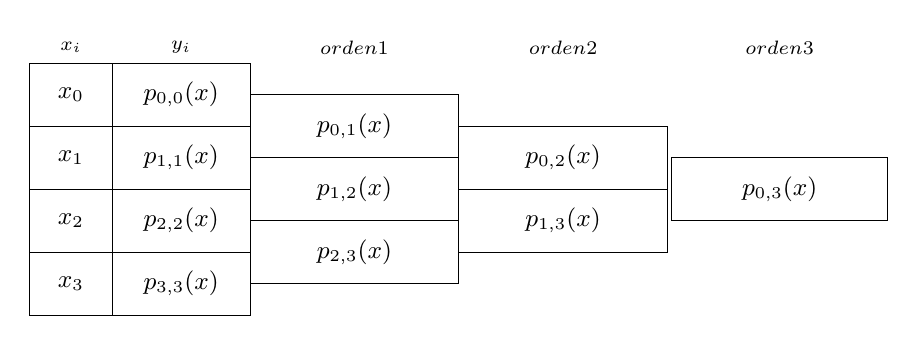
\begin{tikzpicture}[x=1cm,y=1cm]
\path[use as bounding box] (0,-3.65) rectangle (11,-0.0);
\node[font=\scriptsize] at (0.55,-0.25) {$x_i$};
\node[font=\scriptsize] at (1.95,-0.25) {$y_i$};
\node[font=\scriptsize] at (4.15,-0.25) {$\text{orden }1$};
\node[font=\scriptsize] at (6.8,-0.25) {$\text{orden }2$};
\node[font=\scriptsize] at (9.55,-0.25) {$\text{orden }3$};
\node[draw,minimum width=1.05cm,minimum height=.8cm,inner sep=1pt,font=\small] at (0.55,-0.85) {$x_0$};
\node[draw,minimum width=1.05cm,minimum height=.8cm,inner sep=1pt,font=\small] at (0.55,-1.65) {$x_1$};
\node[draw,minimum width=1.05cm,minimum height=.8cm,inner sep=1pt,font=\small] at (0.55,-2.45) {$x_2$};
\node[draw,minimum width=1.05cm,minimum height=.8cm,inner sep=1pt,font=\small] at (0.55,-3.2500000000000004) {$x_3$};
\node[draw,minimum width=1.75cm,minimum height=.8cm,inner sep=1pt,font=\small] at (1.95,-0.85) {$p_{0,0}(x)$};
\node[draw,minimum width=1.75cm,minimum height=.8cm,inner sep=1pt,font=\small] at (1.95,-1.65) {$p_{1,1}(x)$};
\node[draw,minimum width=1.75cm,minimum height=.8cm,inner sep=1pt,font=\small] at (1.95,-2.45) {$p_{2,2}(x)$};
\node[draw,minimum width=1.75cm,minimum height=.8cm,inner sep=1pt,font=\small] at (1.95,-3.2500000000000004) {$p_{3,3}(x)$};
\node[draw,minimum width=2.65cm,minimum height=.8cm,inner sep=1pt,font=\small] at (4.15,-1.25) {$p_{0,1}(x)$};
\node[draw,minimum width=2.65cm,minimum height=.8cm,inner sep=1pt,font=\small] at (4.15,-2.05) {$p_{1,2}(x)$};
\node[draw,minimum width=2.65cm,minimum height=.8cm,inner sep=1pt,font=\small] at (4.15,-2.85) {$p_{2,3}(x)$};
\node[draw,minimum width=2.65cm,minimum height=.8cm,inner sep=1pt,font=\small] at (6.8,-1.65) {$p_{0,2}(x)$};
\node[draw,minimum width=2.65cm,minimum height=.8cm,inner sep=1pt,font=\small] at (6.8,-2.45) {$p_{1,3}(x)$};
\node[draw,minimum width=2.75cm,minimum height=.8cm,inner sep=1pt,font=\small] at (9.55,-2.0500000000000003) {$p_{0,3}(x)$};
\end{tikzpicture}\end{center}
\small\[p_{i,j}(x)=\frac{(x-x_j)p_{i,j-1}(x)+(x_i-x)p_{i+1,j}(x)}{x_i-x_j}.\]
\end{frame}
\begin{frame}[t]{Neville: ejemplo}
\par\noindent\begin{minipage}[t][12mm][t]{\textwidth}\small\strut $f(x)=(x/2)^{x-2}$; $x=5/2$; comenzar con los nodos $1,2$.\end{minipage}\par\nointerlineskip
\begin{center}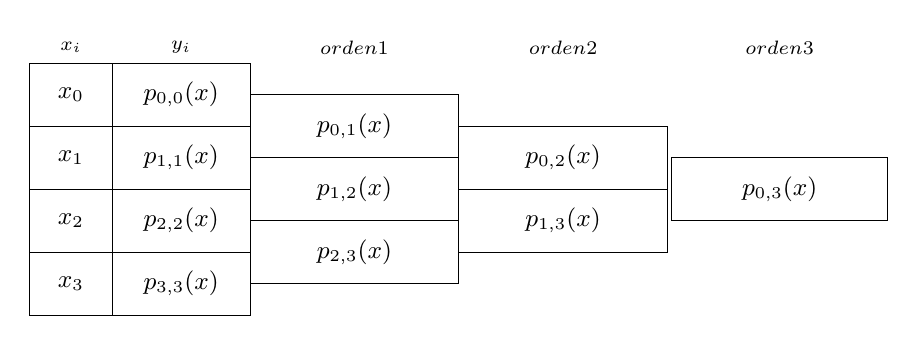
\begin{tikzpicture}[x=1cm,y=1cm]
\path[use as bounding box] (0,-3.65) rectangle (11,-0.0);
\node[font=\scriptsize] at (0.55,-0.25) {$x_i$};
\node[font=\scriptsize] at (1.95,-0.25) {$y_i$};
\node[font=\scriptsize] at (4.15,-0.25) {$\text{orden }1$};
\node[font=\scriptsize] at (6.8,-0.25) {$\text{orden }2$};
\node[font=\scriptsize] at (9.55,-0.25) {$\text{orden }3$};
\node[draw,minimum width=1.05cm,minimum height=.8cm,inner sep=1pt,font=\small] at (0.55,-0.85) {$x_0$};
\node[draw,minimum width=1.05cm,minimum height=.8cm,inner sep=1pt,font=\small] at (0.55,-1.65) {$x_1$};
\node[draw,minimum width=1.05cm,minimum height=.8cm,inner sep=1pt,font=\small] at (0.55,-2.45) {$x_2$};
\node[draw,minimum width=1.05cm,minimum height=.8cm,inner sep=1pt,font=\small] at (0.55,-3.2500000000000004) {$x_3$};
\node[draw,minimum width=1.75cm,minimum height=.8cm,inner sep=1pt,font=\small] at (1.95,-0.85) {$p_{0,0}(x)$};
\node[draw,minimum width=1.75cm,minimum height=.8cm,inner sep=1pt,font=\small] at (1.95,-1.65) {$p_{1,1}(x)$};
\node[draw,minimum width=1.75cm,minimum height=.8cm,inner sep=1pt,font=\small] at (1.95,-2.45) {$p_{2,2}(x)$};
\node[draw,minimum width=1.75cm,minimum height=.8cm,inner sep=1pt,font=\small] at (1.95,-3.2500000000000004) {$p_{3,3}(x)$};
\node[draw,minimum width=2.65cm,minimum height=.8cm,inner sep=1pt,font=\small] at (4.15,-1.25) {$p_{0,1}(x)$};
\node[draw,minimum width=2.65cm,minimum height=.8cm,inner sep=1pt,font=\small] at (4.15,-2.05) {$p_{1,2}(x)$};
\node[draw,minimum width=2.65cm,minimum height=.8cm,inner sep=1pt,font=\small] at (4.15,-2.85) {$p_{2,3}(x)$};
\node[draw,minimum width=2.65cm,minimum height=.8cm,inner sep=1pt,font=\small] at (6.8,-1.65) {$p_{0,2}(x)$};
\node[draw,minimum width=2.65cm,minimum height=.8cm,inner sep=1pt,font=\small] at (6.8,-2.45) {$p_{1,3}(x)$};
\node[draw,minimum width=2.75cm,minimum height=.8cm,inner sep=1pt,font=\small] at (9.55,-2.0500000000000003) {$p_{0,3}(x)$};
\end{tikzpicture}\end{center}
\small\[p_{i,j}(x)=\frac{(x-x_j)p_{i,j-1}(x)+(x_i-x)p_{i+1,j}(x)}{x_i-x_j}.\]
\end{frame}
\begin{frame}[t]{Neville: ejemplo}
\par\noindent\begin{minipage}[t][12mm][t]{\textwidth}\small\strut $f(x)=(x/2)^{x-2}$; evaluar en $x=5/2$; nodos $1,2,3,4$.\end{minipage}\par\nointerlineskip
\begin{center}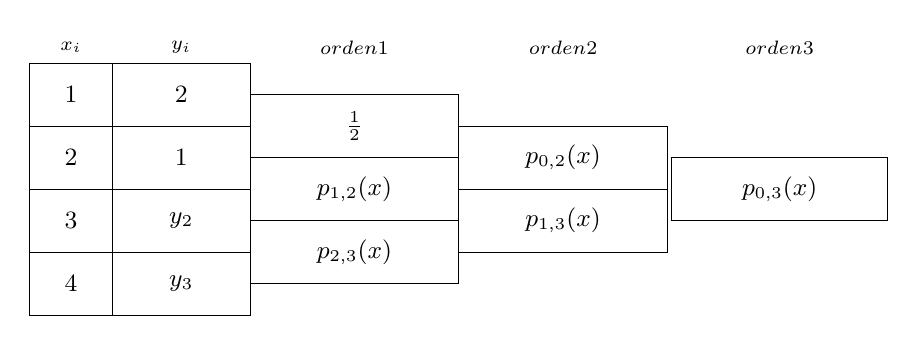
\begin{tikzpicture}[x=1cm,y=1cm]
\path[use as bounding box] (0,-3.65) rectangle (11,-0.0);
\node[font=\scriptsize] at (0.55,-0.25) {$x_i$};
\node[font=\scriptsize] at (1.95,-0.25) {$y_i$};
\node[font=\scriptsize] at (4.15,-0.25) {$\text{orden }1$};
\node[font=\scriptsize] at (6.8,-0.25) {$\text{orden }2$};
\node[font=\scriptsize] at (9.55,-0.25) {$\text{orden }3$};
\node[draw,minimum width=1.05cm,minimum height=.8cm,inner sep=1pt,font=\small] at (0.55,-0.85) {$1$};
\node[draw,minimum width=1.05cm,minimum height=.8cm,inner sep=1pt,font=\small] at (0.55,-1.65) {$2$};
\node[draw,minimum width=1.05cm,minimum height=.8cm,inner sep=1pt,font=\small] at (0.55,-2.45) {$3$};
\node[draw,minimum width=1.05cm,minimum height=.8cm,inner sep=1pt,font=\small] at (0.55,-3.2500000000000004) {$4$};
\node[draw,minimum width=1.75cm,minimum height=.8cm,inner sep=1pt,font=\small] at (1.95,-0.85) {$2$};
\node[draw,minimum width=1.75cm,minimum height=.8cm,inner sep=1pt,font=\small] at (1.95,-1.65) {$1$};
\node[draw,minimum width=1.75cm,minimum height=.8cm,inner sep=1pt,font=\small] at (1.95,-2.45) {$y_2$};
\node[draw,minimum width=1.75cm,minimum height=.8cm,inner sep=1pt,font=\small] at (1.95,-3.2500000000000004) {$y_3$};
\node[draw,minimum width=2.65cm,minimum height=.8cm,inner sep=1pt,font=\small] at (4.15,-1.25) {$\frac12$};
\node[draw,minimum width=2.65cm,minimum height=.8cm,inner sep=1pt,font=\small] at (4.15,-2.05) {$p_{1,2}(x)$};
\node[draw,minimum width=2.65cm,minimum height=.8cm,inner sep=1pt,font=\small] at (4.15,-2.85) {$p_{2,3}(x)$};
\node[draw,minimum width=2.65cm,minimum height=.8cm,inner sep=1pt,font=\small] at (6.8,-1.65) {$p_{0,2}(x)$};
\node[draw,minimum width=2.65cm,minimum height=.8cm,inner sep=1pt,font=\small] at (6.8,-2.45) {$p_{1,3}(x)$};
\node[draw,minimum width=2.75cm,minimum height=.8cm,inner sep=1pt,font=\small] at (9.55,-2.0500000000000003) {$p_{0,3}(x)$};
\end{tikzpicture}\end{center}
\[P_1(5/2)=\frac12.\]
\end{frame}
\begin{frame}[t]{Neville: ejemplo}
\par\noindent\begin{minipage}[t][12mm][t]{\textwidth}\small\strut $f(x)=(x/2)^{x-2}$; evaluar en $x=5/2$; nodos $1,2,3,4$.\end{minipage}\par\nointerlineskip
\begin{center}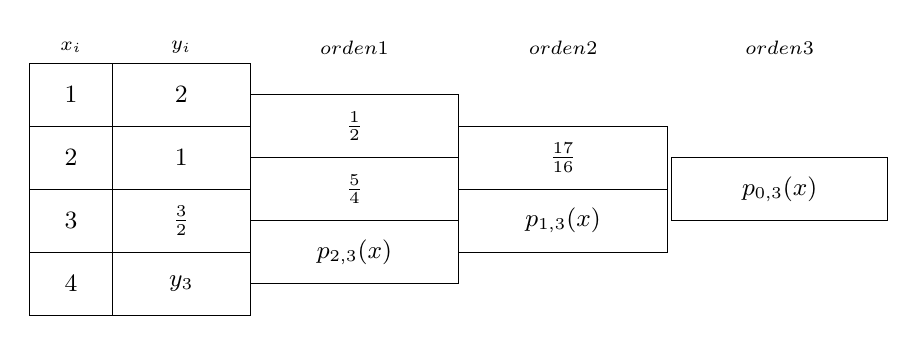
\begin{tikzpicture}[x=1cm,y=1cm]
\path[use as bounding box] (0,-3.65) rectangle (11,-0.0);
\node[font=\scriptsize] at (0.55,-0.25) {$x_i$};
\node[font=\scriptsize] at (1.95,-0.25) {$y_i$};
\node[font=\scriptsize] at (4.15,-0.25) {$\text{orden }1$};
\node[font=\scriptsize] at (6.8,-0.25) {$\text{orden }2$};
\node[font=\scriptsize] at (9.55,-0.25) {$\text{orden }3$};
\node[draw,minimum width=1.05cm,minimum height=.8cm,inner sep=1pt,font=\small] at (0.55,-0.85) {$1$};
\node[draw,minimum width=1.05cm,minimum height=.8cm,inner sep=1pt,font=\small] at (0.55,-1.65) {$2$};
\node[draw,minimum width=1.05cm,minimum height=.8cm,inner sep=1pt,font=\small] at (0.55,-2.45) {$3$};
\node[draw,minimum width=1.05cm,minimum height=.8cm,inner sep=1pt,font=\small] at (0.55,-3.2500000000000004) {$4$};
\node[draw,minimum width=1.75cm,minimum height=.8cm,inner sep=1pt,font=\small] at (1.95,-0.85) {$2$};
\node[draw,minimum width=1.75cm,minimum height=.8cm,inner sep=1pt,font=\small] at (1.95,-1.65) {$1$};
\node[draw,minimum width=1.75cm,minimum height=.8cm,inner sep=1pt,font=\small] at (1.95,-2.45) {$\frac32$};
\node[draw,minimum width=1.75cm,minimum height=.8cm,inner sep=1pt,font=\small] at (1.95,-3.2500000000000004) {$y_3$};
\node[draw,minimum width=2.65cm,minimum height=.8cm,inner sep=1pt,font=\small] at (4.15,-1.25) {$\frac12$};
\node[draw,minimum width=2.65cm,minimum height=.8cm,inner sep=1pt,font=\small] at (4.15,-2.05) {$\frac54$};
\node[draw,minimum width=2.65cm,minimum height=.8cm,inner sep=1pt,font=\small] at (4.15,-2.85) {$p_{2,3}(x)$};
\node[draw,minimum width=2.65cm,minimum height=.8cm,inner sep=1pt,font=\small] at (6.8,-1.65) {$\frac{17}{16}$};
\node[draw,minimum width=2.65cm,minimum height=.8cm,inner sep=1pt,font=\small] at (6.8,-2.45) {$p_{1,3}(x)$};
\node[draw,minimum width=2.75cm,minimum height=.8cm,inner sep=1pt,font=\small] at (9.55,-2.0500000000000003) {$p_{0,3}(x)$};
\end{tikzpicture}\end{center}
\[P_1(5/2)=\frac12,\quad P_2(5/2)=\frac{17}{16}.\]
\end{frame}
\begin{frame}[t]{Neville: ejemplo}
\par\noindent\begin{minipage}[t][12mm][t]{\textwidth}\small\strut $f(x)=(x/2)^{x-2}$; evaluar en $x=5/2$; nodos $1,2,3,4$.\end{minipage}\par\nointerlineskip
\begin{center}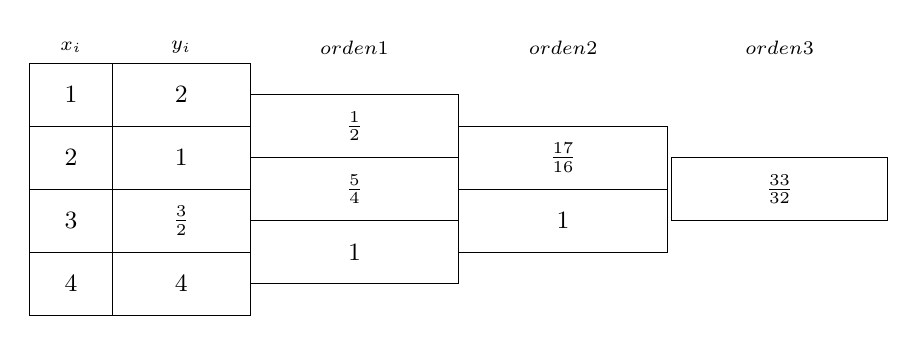
\begin{tikzpicture}[x=1cm,y=1cm]
\path[use as bounding box] (0,-3.65) rectangle (11,-0.0);
\node[font=\scriptsize] at (0.55,-0.25) {$x_i$};
\node[font=\scriptsize] at (1.95,-0.25) {$y_i$};
\node[font=\scriptsize] at (4.15,-0.25) {$\text{orden }1$};
\node[font=\scriptsize] at (6.8,-0.25) {$\text{orden }2$};
\node[font=\scriptsize] at (9.55,-0.25) {$\text{orden }3$};
\node[draw,minimum width=1.05cm,minimum height=.8cm,inner sep=1pt,font=\small] at (0.55,-0.85) {$1$};
\node[draw,minimum width=1.05cm,minimum height=.8cm,inner sep=1pt,font=\small] at (0.55,-1.65) {$2$};
\node[draw,minimum width=1.05cm,minimum height=.8cm,inner sep=1pt,font=\small] at (0.55,-2.45) {$3$};
\node[draw,minimum width=1.05cm,minimum height=.8cm,inner sep=1pt,font=\small] at (0.55,-3.2500000000000004) {$4$};
\node[draw,minimum width=1.75cm,minimum height=.8cm,inner sep=1pt,font=\small] at (1.95,-0.85) {$2$};
\node[draw,minimum width=1.75cm,minimum height=.8cm,inner sep=1pt,font=\small] at (1.95,-1.65) {$1$};
\node[draw,minimum width=1.75cm,minimum height=.8cm,inner sep=1pt,font=\small] at (1.95,-2.45) {$\frac32$};
\node[draw,minimum width=1.75cm,minimum height=.8cm,inner sep=1pt,font=\small] at (1.95,-3.2500000000000004) {$4$};
\node[draw,minimum width=2.65cm,minimum height=.8cm,inner sep=1pt,font=\small] at (4.15,-1.25) {$\frac12$};
\node[draw,minimum width=2.65cm,minimum height=.8cm,inner sep=1pt,font=\small] at (4.15,-2.05) {$\frac54$};
\node[draw,minimum width=2.65cm,minimum height=.8cm,inner sep=1pt,font=\small] at (4.15,-2.85) {$1$};
\node[draw,minimum width=2.65cm,minimum height=.8cm,inner sep=1pt,font=\small] at (6.8,-1.65) {$\frac{17}{16}$};
\node[draw,minimum width=2.65cm,minimum height=.8cm,inner sep=1pt,font=\small] at (6.8,-2.45) {$1$};
\node[draw,minimum width=2.75cm,minimum height=.8cm,inner sep=1pt,font=\small] at (9.55,-2.0500000000000003) {$\frac{33}{32}$};
\end{tikzpicture}\end{center}
\[P_1(5/2)=\frac12,\quad P_2(5/2)=\frac{17}{16},\quad P_3(5/2)=\frac{33}{32}.\]
\end{frame}
\begin{frame}[t]{Diferencias divididas}
Desarrollar una expresión explícita a partir de las tablas anteriores puede resultar laborioso.
\bigskip
El método de diferencias divididas permite construir directamente una expresión del polinomio interpolante.
\end{frame}
\begin{frame}[t]{Forma explícita del polinomio}
La expresión explícita del interpolante es útil cuando se pretende derivarlo, integrarlo u operar con él.
\bigskip
Las diferencias divididas proporcionan los coeficientes de la forma de Newton.
\end{frame}
\begin{frame}[t]{Forma de Newton}
\small\[P_n(x)=f[x_0]+\sum_{k=1}^n f[x_0,\ldots,x_k]\prod_{j=0}^{k-1}(x-x_j).\]Las diferencias divididas se definen por:\[f[x_i]=f(x_i).\]\[f[x_i,x_{i+1}]=\frac{f(x_{i+1})-f(x_i)}{x_{i+1}-x_i}.\]\[f[x_i,\ldots,x_{i+k}]=\frac{f[x_{i+1},\ldots,x_{i+k}]-f[x_i,\ldots,x_{i+k-1}]}{x_{i+k}-x_i}.\]
\end{frame}
\begin{frame}[t]{Diferencias divididas: pirámide}
\par\noindent\begin{minipage}[t][12mm][t]{\textwidth}\small\strut Pirámide para construir $P_3(x)$.\end{minipage}\par\nointerlineskip
\begin{center}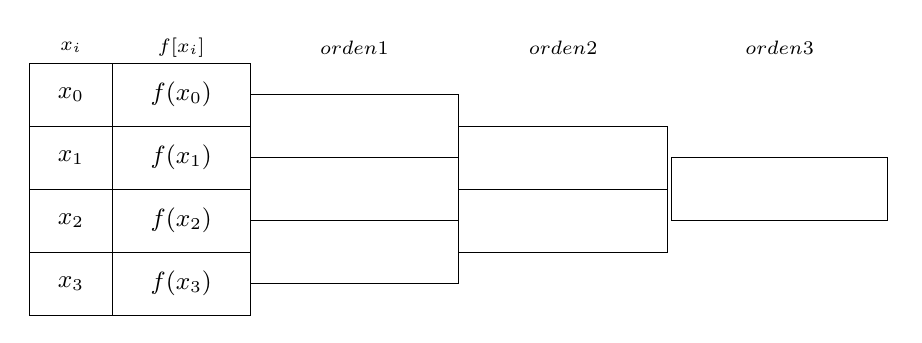
\begin{tikzpicture}[x=1cm,y=1cm]
\path[use as bounding box] (0,-3.65) rectangle (11,-0.0);
\node[font=\scriptsize] at (0.55,-0.25) {$x_i$};
\node[font=\scriptsize] at (1.95,-0.25) {$f[x_i]$};
\node[font=\scriptsize] at (4.15,-0.25) {$\text{orden }1$};
\node[font=\scriptsize] at (6.8,-0.25) {$\text{orden }2$};
\node[font=\scriptsize] at (9.55,-0.25) {$\text{orden }3$};
\node[draw,minimum width=1.05cm,minimum height=.8cm,inner sep=1pt,font=\small] at (0.55,-0.85) {$x_0$};
\node[draw,minimum width=1.05cm,minimum height=.8cm,inner sep=1pt,font=\small] at (0.55,-1.65) {$x_1$};
\node[draw,minimum width=1.05cm,minimum height=.8cm,inner sep=1pt,font=\small] at (0.55,-2.45) {$x_2$};
\node[draw,minimum width=1.05cm,minimum height=.8cm,inner sep=1pt,font=\small] at (0.55,-3.2500000000000004) {$x_3$};
\node[draw,minimum width=1.75cm,minimum height=.8cm,inner sep=1pt,font=\small] at (1.95,-0.85) {$f(x_0)$};
\node[draw,minimum width=1.75cm,minimum height=.8cm,inner sep=1pt,font=\small] at (1.95,-1.65) {$f(x_1)$};
\node[draw,minimum width=1.75cm,minimum height=.8cm,inner sep=1pt,font=\small] at (1.95,-2.45) {$f(x_2)$};
\node[draw,minimum width=1.75cm,minimum height=.8cm,inner sep=1pt,font=\small] at (1.95,-3.2500000000000004) {$f(x_3)$};
\node[draw,minimum width=2.65cm,minimum height=.8cm,inner sep=1pt,font=\small] at (4.15,-1.25) {$$};
\node[draw,minimum width=2.65cm,minimum height=.8cm,inner sep=1pt,font=\small] at (4.15,-2.05) {$$};
\node[draw,minimum width=2.65cm,minimum height=.8cm,inner sep=1pt,font=\small] at (4.15,-2.85) {$$};
\node[draw,minimum width=2.65cm,minimum height=.8cm,inner sep=1pt,font=\small] at (6.8,-1.65) {$$};
\node[draw,minimum width=2.65cm,minimum height=.8cm,inner sep=1pt,font=\small] at (6.8,-2.45) {$$};
\node[draw,minimum width=2.75cm,minimum height=.8cm,inner sep=1pt,font=\small] at (9.55,-2.0500000000000003) {$$};
\end{tikzpicture}\end{center}
\[f[x_i]=f(x_i).\]
\end{frame}
\begin{frame}[t]{Diferencias divididas: pirámide}
\par\noindent\begin{minipage}[t][12mm][t]{\textwidth}\small\strut Pirámide para construir $P_3(x)$.\end{minipage}\par\nointerlineskip
\begin{center}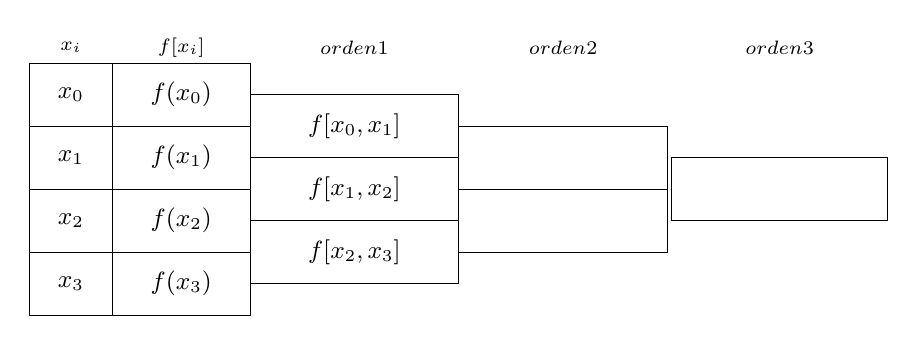
\begin{tikzpicture}[x=1cm,y=1cm]
\path[use as bounding box] (0,-3.65) rectangle (11,-0.0);
\node[font=\scriptsize] at (0.55,-0.25) {$x_i$};
\node[font=\scriptsize] at (1.95,-0.25) {$f[x_i]$};
\node[font=\scriptsize] at (4.15,-0.25) {$\text{orden }1$};
\node[font=\scriptsize] at (6.8,-0.25) {$\text{orden }2$};
\node[font=\scriptsize] at (9.55,-0.25) {$\text{orden }3$};
\node[draw,minimum width=1.05cm,minimum height=.8cm,inner sep=1pt,font=\small] at (0.55,-0.85) {$x_0$};
\node[draw,minimum width=1.05cm,minimum height=.8cm,inner sep=1pt,font=\small] at (0.55,-1.65) {$x_1$};
\node[draw,minimum width=1.05cm,minimum height=.8cm,inner sep=1pt,font=\small] at (0.55,-2.45) {$x_2$};
\node[draw,minimum width=1.05cm,minimum height=.8cm,inner sep=1pt,font=\small] at (0.55,-3.2500000000000004) {$x_3$};
\node[draw,minimum width=1.75cm,minimum height=.8cm,inner sep=1pt,font=\small] at (1.95,-0.85) {$f(x_0)$};
\node[draw,minimum width=1.75cm,minimum height=.8cm,inner sep=1pt,font=\small] at (1.95,-1.65) {$f(x_1)$};
\node[draw,minimum width=1.75cm,minimum height=.8cm,inner sep=1pt,font=\small] at (1.95,-2.45) {$f(x_2)$};
\node[draw,minimum width=1.75cm,minimum height=.8cm,inner sep=1pt,font=\small] at (1.95,-3.2500000000000004) {$f(x_3)$};
\node[draw,minimum width=2.65cm,minimum height=.8cm,inner sep=1pt,font=\small] at (4.15,-1.25) {$f[x_0,x_1]$};
\node[draw,minimum width=2.65cm,minimum height=.8cm,inner sep=1pt,font=\small] at (4.15,-2.05) {$f[x_1,x_2]$};
\node[draw,minimum width=2.65cm,minimum height=.8cm,inner sep=1pt,font=\small] at (4.15,-2.85) {$f[x_2,x_3]$};
\node[draw,minimum width=2.65cm,minimum height=.8cm,inner sep=1pt,font=\small] at (6.8,-1.65) {$$};
\node[draw,minimum width=2.65cm,minimum height=.8cm,inner sep=1pt,font=\small] at (6.8,-2.45) {$$};
\node[draw,minimum width=2.75cm,minimum height=.8cm,inner sep=1pt,font=\small] at (9.55,-2.0500000000000003) {$$};
\end{tikzpicture}\end{center}
\small\[f[x_i,x_{i+1}]=\frac{f[x_{i+1}]-f[x_i]}{x_{i+1}-x_i}.\]
\end{frame}
\begin{frame}[t]{Diferencias divididas: primer orden}
\par\noindent\begin{minipage}[t][12mm][t]{\textwidth}\small\strut Pirámide para construir $P_3(x)$.\end{minipage}\par\nointerlineskip
\begin{center}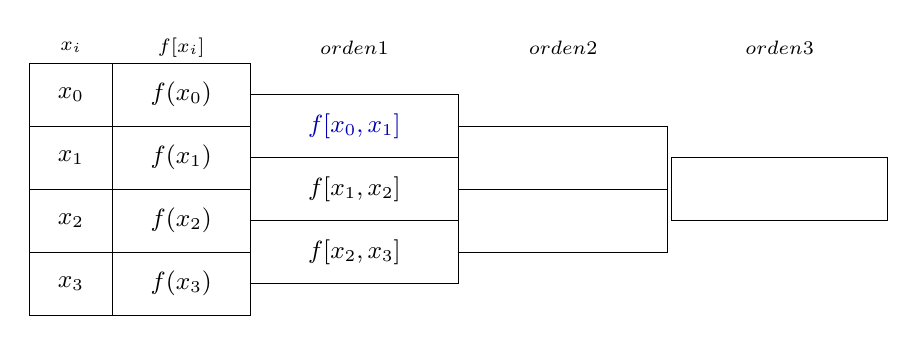
\begin{tikzpicture}[x=1cm,y=1cm]
\path[use as bounding box] (0,-3.65) rectangle (11,-0.0);
\node[font=\scriptsize] at (0.55,-0.25) {$x_i$};
\node[font=\scriptsize] at (1.95,-0.25) {$f[x_i]$};
\node[font=\scriptsize] at (4.15,-0.25) {$\text{orden }1$};
\node[font=\scriptsize] at (6.8,-0.25) {$\text{orden }2$};
\node[font=\scriptsize] at (9.55,-0.25) {$\text{orden }3$};
\node[draw,minimum width=1.05cm,minimum height=.8cm,inner sep=1pt,font=\small] at (0.55,-0.85) {$x_0$};
\node[draw,minimum width=1.05cm,minimum height=.8cm,inner sep=1pt,font=\small] at (0.55,-1.65) {$x_1$};
\node[draw,minimum width=1.05cm,minimum height=.8cm,inner sep=1pt,font=\small] at (0.55,-2.45) {$x_2$};
\node[draw,minimum width=1.05cm,minimum height=.8cm,inner sep=1pt,font=\small] at (0.55,-3.2500000000000004) {$x_3$};
\node[draw,minimum width=1.75cm,minimum height=.8cm,inner sep=1pt,font=\small] at (1.95,-0.85) {$f(x_0)$};
\node[draw,minimum width=1.75cm,minimum height=.8cm,inner sep=1pt,font=\small] at (1.95,-1.65) {$f(x_1)$};
\node[draw,minimum width=1.75cm,minimum height=.8cm,inner sep=1pt,font=\small] at (1.95,-2.45) {$f(x_2)$};
\node[draw,minimum width=1.75cm,minimum height=.8cm,inner sep=1pt,font=\small] at (1.95,-3.2500000000000004) {$f(x_3)$};
\node[draw,minimum width=2.65cm,minimum height=.8cm,inner sep=1pt,font=\small,text=blue!70!black] at (4.15,-1.25) {$f[x_0,x_1]$};
\node[draw,minimum width=2.65cm,minimum height=.8cm,inner sep=1pt,font=\small] at (4.15,-2.05) {$f[x_1,x_2]$};
\node[draw,minimum width=2.65cm,minimum height=.8cm,inner sep=1pt,font=\small] at (4.15,-2.85) {$f[x_2,x_3]$};
\node[draw,minimum width=2.65cm,minimum height=.8cm,inner sep=1pt,font=\small] at (6.8,-1.65) {$$};
\node[draw,minimum width=2.65cm,minimum height=.8cm,inner sep=1pt,font=\small] at (6.8,-2.45) {$$};
\node[draw,minimum width=2.75cm,minimum height=.8cm,inner sep=1pt,font=\small] at (9.55,-2.0500000000000003) {$$};
\end{tikzpicture}\end{center}
\small\[f[x_0,x_1]=\frac{f(x_1)-f(x_0)}{x_1-x_0}.\]
\end{frame}
\begin{frame}[t]{Diferencias divididas: primer orden}
\par\noindent\begin{minipage}[t][12mm][t]{\textwidth}\small\strut Pirámide para construir $P_3(x)$.\end{minipage}\par\nointerlineskip
\begin{center}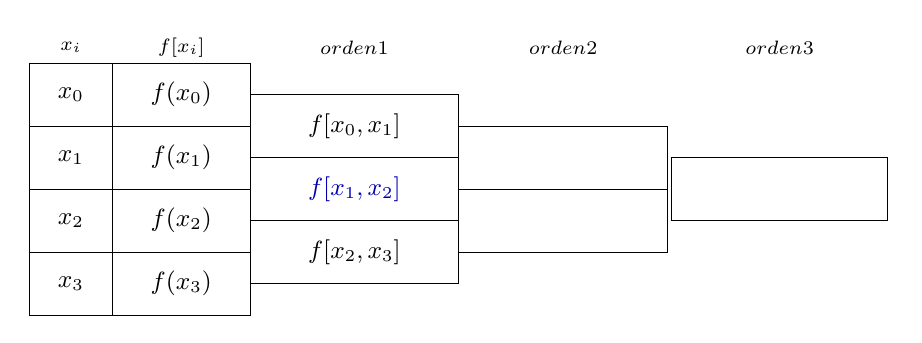
\begin{tikzpicture}[x=1cm,y=1cm]
\path[use as bounding box] (0,-3.65) rectangle (11,-0.0);
\node[font=\scriptsize] at (0.55,-0.25) {$x_i$};
\node[font=\scriptsize] at (1.95,-0.25) {$f[x_i]$};
\node[font=\scriptsize] at (4.15,-0.25) {$\text{orden }1$};
\node[font=\scriptsize] at (6.8,-0.25) {$\text{orden }2$};
\node[font=\scriptsize] at (9.55,-0.25) {$\text{orden }3$};
\node[draw,minimum width=1.05cm,minimum height=.8cm,inner sep=1pt,font=\small] at (0.55,-0.85) {$x_0$};
\node[draw,minimum width=1.05cm,minimum height=.8cm,inner sep=1pt,font=\small] at (0.55,-1.65) {$x_1$};
\node[draw,minimum width=1.05cm,minimum height=.8cm,inner sep=1pt,font=\small] at (0.55,-2.45) {$x_2$};
\node[draw,minimum width=1.05cm,minimum height=.8cm,inner sep=1pt,font=\small] at (0.55,-3.2500000000000004) {$x_3$};
\node[draw,minimum width=1.75cm,minimum height=.8cm,inner sep=1pt,font=\small] at (1.95,-0.85) {$f(x_0)$};
\node[draw,minimum width=1.75cm,minimum height=.8cm,inner sep=1pt,font=\small] at (1.95,-1.65) {$f(x_1)$};
\node[draw,minimum width=1.75cm,minimum height=.8cm,inner sep=1pt,font=\small] at (1.95,-2.45) {$f(x_2)$};
\node[draw,minimum width=1.75cm,minimum height=.8cm,inner sep=1pt,font=\small] at (1.95,-3.2500000000000004) {$f(x_3)$};
\node[draw,minimum width=2.65cm,minimum height=.8cm,inner sep=1pt,font=\small] at (4.15,-1.25) {$f[x_0,x_1]$};
\node[draw,minimum width=2.65cm,minimum height=.8cm,inner sep=1pt,font=\small,text=blue!70!black] at (4.15,-2.05) {$f[x_1,x_2]$};
\node[draw,minimum width=2.65cm,minimum height=.8cm,inner sep=1pt,font=\small] at (4.15,-2.85) {$f[x_2,x_3]$};
\node[draw,minimum width=2.65cm,minimum height=.8cm,inner sep=1pt,font=\small] at (6.8,-1.65) {$$};
\node[draw,minimum width=2.65cm,minimum height=.8cm,inner sep=1pt,font=\small] at (6.8,-2.45) {$$};
\node[draw,minimum width=2.75cm,minimum height=.8cm,inner sep=1pt,font=\small] at (9.55,-2.0500000000000003) {$$};
\end{tikzpicture}\end{center}
\small\[f[x_1,x_2]=\frac{f(x_2)-f(x_1)}{x_2-x_1}.\]
\end{frame}
\begin{frame}[t]{Diferencias divididas: primer orden}
\par\noindent\begin{minipage}[t][12mm][t]{\textwidth}\small\strut Pirámide para construir $P_3(x)$.\end{minipage}\par\nointerlineskip
\begin{center}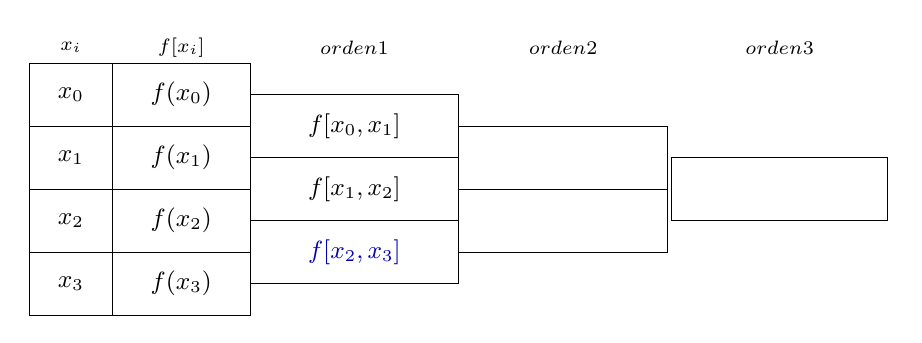
\begin{tikzpicture}[x=1cm,y=1cm]
\path[use as bounding box] (0,-3.65) rectangle (11,-0.0);
\node[font=\scriptsize] at (0.55,-0.25) {$x_i$};
\node[font=\scriptsize] at (1.95,-0.25) {$f[x_i]$};
\node[font=\scriptsize] at (4.15,-0.25) {$\text{orden }1$};
\node[font=\scriptsize] at (6.8,-0.25) {$\text{orden }2$};
\node[font=\scriptsize] at (9.55,-0.25) {$\text{orden }3$};
\node[draw,minimum width=1.05cm,minimum height=.8cm,inner sep=1pt,font=\small] at (0.55,-0.85) {$x_0$};
\node[draw,minimum width=1.05cm,minimum height=.8cm,inner sep=1pt,font=\small] at (0.55,-1.65) {$x_1$};
\node[draw,minimum width=1.05cm,minimum height=.8cm,inner sep=1pt,font=\small] at (0.55,-2.45) {$x_2$};
\node[draw,minimum width=1.05cm,minimum height=.8cm,inner sep=1pt,font=\small] at (0.55,-3.2500000000000004) {$x_3$};
\node[draw,minimum width=1.75cm,minimum height=.8cm,inner sep=1pt,font=\small] at (1.95,-0.85) {$f(x_0)$};
\node[draw,minimum width=1.75cm,minimum height=.8cm,inner sep=1pt,font=\small] at (1.95,-1.65) {$f(x_1)$};
\node[draw,minimum width=1.75cm,minimum height=.8cm,inner sep=1pt,font=\small] at (1.95,-2.45) {$f(x_2)$};
\node[draw,minimum width=1.75cm,minimum height=.8cm,inner sep=1pt,font=\small] at (1.95,-3.2500000000000004) {$f(x_3)$};
\node[draw,minimum width=2.65cm,minimum height=.8cm,inner sep=1pt,font=\small] at (4.15,-1.25) {$f[x_0,x_1]$};
\node[draw,minimum width=2.65cm,minimum height=.8cm,inner sep=1pt,font=\small] at (4.15,-2.05) {$f[x_1,x_2]$};
\node[draw,minimum width=2.65cm,minimum height=.8cm,inner sep=1pt,font=\small,text=blue!70!black] at (4.15,-2.85) {$f[x_2,x_3]$};
\node[draw,minimum width=2.65cm,minimum height=.8cm,inner sep=1pt,font=\small] at (6.8,-1.65) {$$};
\node[draw,minimum width=2.65cm,minimum height=.8cm,inner sep=1pt,font=\small] at (6.8,-2.45) {$$};
\node[draw,minimum width=2.75cm,minimum height=.8cm,inner sep=1pt,font=\small] at (9.55,-2.0500000000000003) {$$};
\end{tikzpicture}\end{center}
\small\[f[x_2,x_3]=\frac{f(x_3)-f(x_2)}{x_3-x_2}.\]
\end{frame}
\begin{frame}[t]{Diferencias divididas: segundo orden}
\par\noindent\begin{minipage}[t][12mm][t]{\textwidth}\small\strut Pirámide para construir $P_3(x)$.\end{minipage}\par\nointerlineskip
\begin{center}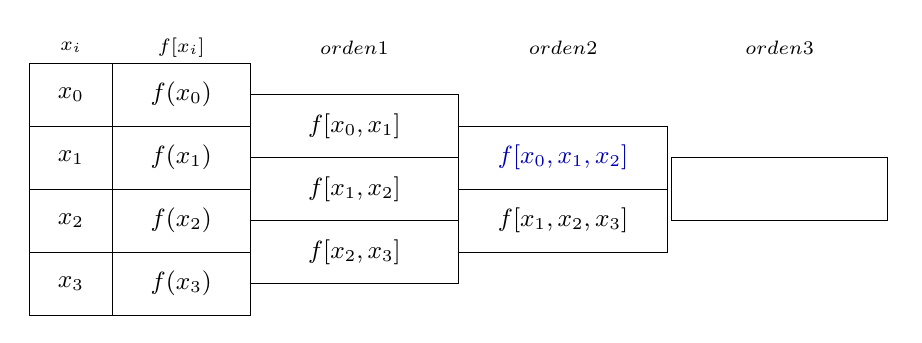
\begin{tikzpicture}[x=1cm,y=1cm]
\path[use as bounding box] (0,-3.65) rectangle (11,-0.0);
\node[font=\scriptsize] at (0.55,-0.25) {$x_i$};
\node[font=\scriptsize] at (1.95,-0.25) {$f[x_i]$};
\node[font=\scriptsize] at (4.15,-0.25) {$\text{orden }1$};
\node[font=\scriptsize] at (6.8,-0.25) {$\text{orden }2$};
\node[font=\scriptsize] at (9.55,-0.25) {$\text{orden }3$};
\node[draw,minimum width=1.05cm,minimum height=.8cm,inner sep=1pt,font=\small] at (0.55,-0.85) {$x_0$};
\node[draw,minimum width=1.05cm,minimum height=.8cm,inner sep=1pt,font=\small] at (0.55,-1.65) {$x_1$};
\node[draw,minimum width=1.05cm,minimum height=.8cm,inner sep=1pt,font=\small] at (0.55,-2.45) {$x_2$};
\node[draw,minimum width=1.05cm,minimum height=.8cm,inner sep=1pt,font=\small] at (0.55,-3.2500000000000004) {$x_3$};
\node[draw,minimum width=1.75cm,minimum height=.8cm,inner sep=1pt,font=\small] at (1.95,-0.85) {$f(x_0)$};
\node[draw,minimum width=1.75cm,minimum height=.8cm,inner sep=1pt,font=\small] at (1.95,-1.65) {$f(x_1)$};
\node[draw,minimum width=1.75cm,minimum height=.8cm,inner sep=1pt,font=\small] at (1.95,-2.45) {$f(x_2)$};
\node[draw,minimum width=1.75cm,minimum height=.8cm,inner sep=1pt,font=\small] at (1.95,-3.2500000000000004) {$f(x_3)$};
\node[draw,minimum width=2.65cm,minimum height=.8cm,inner sep=1pt,font=\small] at (4.15,-1.25) {$f[x_0,x_1]$};
\node[draw,minimum width=2.65cm,minimum height=.8cm,inner sep=1pt,font=\small] at (4.15,-2.05) {$f[x_1,x_2]$};
\node[draw,minimum width=2.65cm,minimum height=.8cm,inner sep=1pt,font=\small] at (4.15,-2.85) {$f[x_2,x_3]$};
\node[draw,minimum width=2.65cm,minimum height=.8cm,inner sep=1pt,font=\small,text=blue!70!black] at (6.8,-1.65) {$f[x_0,x_1,x_2]$};
\node[draw,minimum width=2.65cm,minimum height=.8cm,inner sep=1pt,font=\small] at (6.8,-2.45) {$f[x_1,x_2,x_3]$};
\node[draw,minimum width=2.75cm,minimum height=.8cm,inner sep=1pt,font=\small] at (9.55,-2.0500000000000003) {$$};
\end{tikzpicture}\end{center}
\small\[f[x_0,x_1,x_2]=\frac{f[x_1,x_2]-f[x_0,x_1]}{x_2-x_0}.\]
\end{frame}
\begin{frame}[t]{Diferencias divididas: segundo orden}
\par\noindent\begin{minipage}[t][12mm][t]{\textwidth}\small\strut Pirámide para construir $P_3(x)$.\end{minipage}\par\nointerlineskip
\begin{center}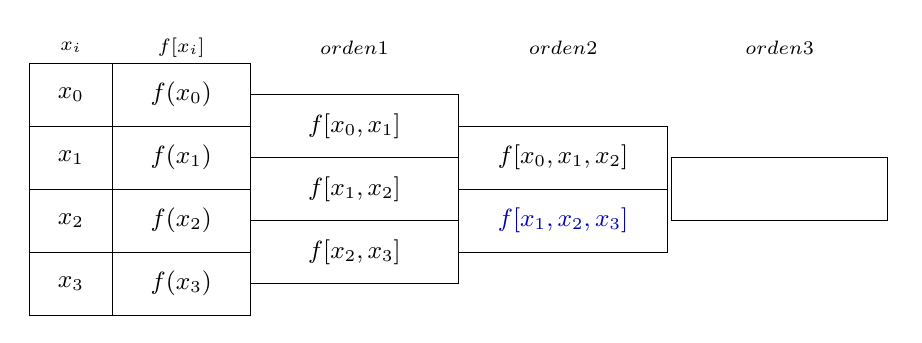
\begin{tikzpicture}[x=1cm,y=1cm]
\path[use as bounding box] (0,-3.65) rectangle (11,-0.0);
\node[font=\scriptsize] at (0.55,-0.25) {$x_i$};
\node[font=\scriptsize] at (1.95,-0.25) {$f[x_i]$};
\node[font=\scriptsize] at (4.15,-0.25) {$\text{orden }1$};
\node[font=\scriptsize] at (6.8,-0.25) {$\text{orden }2$};
\node[font=\scriptsize] at (9.55,-0.25) {$\text{orden }3$};
\node[draw,minimum width=1.05cm,minimum height=.8cm,inner sep=1pt,font=\small] at (0.55,-0.85) {$x_0$};
\node[draw,minimum width=1.05cm,minimum height=.8cm,inner sep=1pt,font=\small] at (0.55,-1.65) {$x_1$};
\node[draw,minimum width=1.05cm,minimum height=.8cm,inner sep=1pt,font=\small] at (0.55,-2.45) {$x_2$};
\node[draw,minimum width=1.05cm,minimum height=.8cm,inner sep=1pt,font=\small] at (0.55,-3.2500000000000004) {$x_3$};
\node[draw,minimum width=1.75cm,minimum height=.8cm,inner sep=1pt,font=\small] at (1.95,-0.85) {$f(x_0)$};
\node[draw,minimum width=1.75cm,minimum height=.8cm,inner sep=1pt,font=\small] at (1.95,-1.65) {$f(x_1)$};
\node[draw,minimum width=1.75cm,minimum height=.8cm,inner sep=1pt,font=\small] at (1.95,-2.45) {$f(x_2)$};
\node[draw,minimum width=1.75cm,minimum height=.8cm,inner sep=1pt,font=\small] at (1.95,-3.2500000000000004) {$f(x_3)$};
\node[draw,minimum width=2.65cm,minimum height=.8cm,inner sep=1pt,font=\small] at (4.15,-1.25) {$f[x_0,x_1]$};
\node[draw,minimum width=2.65cm,minimum height=.8cm,inner sep=1pt,font=\small] at (4.15,-2.05) {$f[x_1,x_2]$};
\node[draw,minimum width=2.65cm,minimum height=.8cm,inner sep=1pt,font=\small] at (4.15,-2.85) {$f[x_2,x_3]$};
\node[draw,minimum width=2.65cm,minimum height=.8cm,inner sep=1pt,font=\small] at (6.8,-1.65) {$f[x_0,x_1,x_2]$};
\node[draw,minimum width=2.65cm,minimum height=.8cm,inner sep=1pt,font=\small,text=blue!70!black] at (6.8,-2.45) {$f[x_1,x_2,x_3]$};
\node[draw,minimum width=2.75cm,minimum height=.8cm,inner sep=1pt,font=\small] at (9.55,-2.0500000000000003) {$$};
\end{tikzpicture}\end{center}
\small\[f[x_1,x_2,x_3]=\frac{f[x_2,x_3]-f[x_1,x_2]}{x_3-x_1}.\]
\end{frame}
\begin{frame}[t]{Diferencias divididas: tercer orden}
\par\noindent\begin{minipage}[t][12mm][t]{\textwidth}\small\strut Pirámide para construir $P_3(x)$.\end{minipage}\par\nointerlineskip
\begin{center}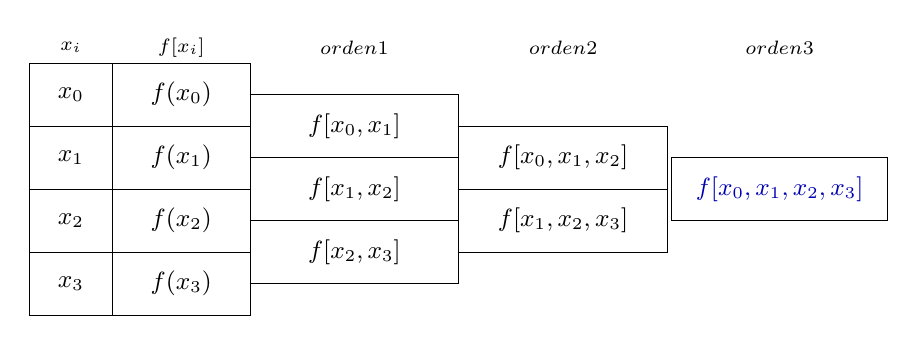
\begin{tikzpicture}[x=1cm,y=1cm]
\path[use as bounding box] (0,-3.65) rectangle (11,-0.0);
\node[font=\scriptsize] at (0.55,-0.25) {$x_i$};
\node[font=\scriptsize] at (1.95,-0.25) {$f[x_i]$};
\node[font=\scriptsize] at (4.15,-0.25) {$\text{orden }1$};
\node[font=\scriptsize] at (6.8,-0.25) {$\text{orden }2$};
\node[font=\scriptsize] at (9.55,-0.25) {$\text{orden }3$};
\node[draw,minimum width=1.05cm,minimum height=.8cm,inner sep=1pt,font=\small] at (0.55,-0.85) {$x_0$};
\node[draw,minimum width=1.05cm,minimum height=.8cm,inner sep=1pt,font=\small] at (0.55,-1.65) {$x_1$};
\node[draw,minimum width=1.05cm,minimum height=.8cm,inner sep=1pt,font=\small] at (0.55,-2.45) {$x_2$};
\node[draw,minimum width=1.05cm,minimum height=.8cm,inner sep=1pt,font=\small] at (0.55,-3.2500000000000004) {$x_3$};
\node[draw,minimum width=1.75cm,minimum height=.8cm,inner sep=1pt,font=\small] at (1.95,-0.85) {$f(x_0)$};
\node[draw,minimum width=1.75cm,minimum height=.8cm,inner sep=1pt,font=\small] at (1.95,-1.65) {$f(x_1)$};
\node[draw,minimum width=1.75cm,minimum height=.8cm,inner sep=1pt,font=\small] at (1.95,-2.45) {$f(x_2)$};
\node[draw,minimum width=1.75cm,minimum height=.8cm,inner sep=1pt,font=\small] at (1.95,-3.2500000000000004) {$f(x_3)$};
\node[draw,minimum width=2.65cm,minimum height=.8cm,inner sep=1pt,font=\small] at (4.15,-1.25) {$f[x_0,x_1]$};
\node[draw,minimum width=2.65cm,minimum height=.8cm,inner sep=1pt,font=\small] at (4.15,-2.05) {$f[x_1,x_2]$};
\node[draw,minimum width=2.65cm,minimum height=.8cm,inner sep=1pt,font=\small] at (4.15,-2.85) {$f[x_2,x_3]$};
\node[draw,minimum width=2.65cm,minimum height=.8cm,inner sep=1pt,font=\small] at (6.8,-1.65) {$f[x_0,x_1,x_2]$};
\node[draw,minimum width=2.65cm,minimum height=.8cm,inner sep=1pt,font=\small] at (6.8,-2.45) {$f[x_1,x_2,x_3]$};
\node[draw,minimum width=2.75cm,minimum height=.8cm,inner sep=1pt,font=\small,text=blue!70!black] at (9.55,-2.0500000000000003) {$f[x_0,x_1,x_2,x_3]$};
\end{tikzpicture}\end{center}
\small\[f[x_0,x_1,x_2,x_3]=\frac{f[x_1,x_2,x_3]-f[x_0,x_1,x_2]}{x_3-x_0}.\]
\end{frame}
\begin{frame}[t]{Coeficientes de Newton}
\par\noindent\begin{minipage}[t][12mm][t]{\textwidth}\small\strut Los coeficientes se leen en el borde superior del triángulo.\end{minipage}\par\nointerlineskip
\begin{center}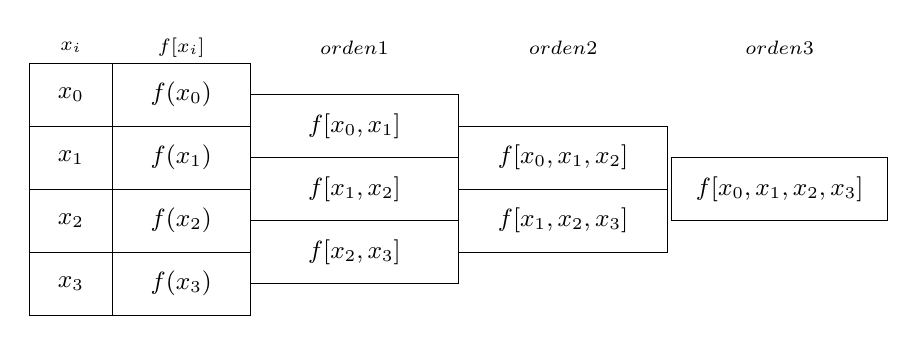
\begin{tikzpicture}[x=1cm,y=1cm]
\path[use as bounding box] (0,-3.65) rectangle (11,-0.0);
\node[font=\scriptsize] at (0.55,-0.25) {$x_i$};
\node[font=\scriptsize] at (1.95,-0.25) {$f[x_i]$};
\node[font=\scriptsize] at (4.15,-0.25) {$\text{orden }1$};
\node[font=\scriptsize] at (6.8,-0.25) {$\text{orden }2$};
\node[font=\scriptsize] at (9.55,-0.25) {$\text{orden }3$};
\node[draw,minimum width=1.05cm,minimum height=.8cm,inner sep=1pt,font=\small] at (0.55,-0.85) {$x_0$};
\node[draw,minimum width=1.05cm,minimum height=.8cm,inner sep=1pt,font=\small] at (0.55,-1.65) {$x_1$};
\node[draw,minimum width=1.05cm,minimum height=.8cm,inner sep=1pt,font=\small] at (0.55,-2.45) {$x_2$};
\node[draw,minimum width=1.05cm,minimum height=.8cm,inner sep=1pt,font=\small] at (0.55,-3.2500000000000004) {$x_3$};
\node[draw,minimum width=1.75cm,minimum height=.8cm,inner sep=1pt,font=\small] at (1.95,-0.85) {$f(x_0)$};
\node[draw,minimum width=1.75cm,minimum height=.8cm,inner sep=1pt,font=\small] at (1.95,-1.65) {$f(x_1)$};
\node[draw,minimum width=1.75cm,minimum height=.8cm,inner sep=1pt,font=\small] at (1.95,-2.45) {$f(x_2)$};
\node[draw,minimum width=1.75cm,minimum height=.8cm,inner sep=1pt,font=\small] at (1.95,-3.2500000000000004) {$f(x_3)$};
\node[draw,minimum width=2.65cm,minimum height=.8cm,inner sep=1pt,font=\small] at (4.15,-1.25) {$f[x_0,x_1]$};
\node[draw,minimum width=2.65cm,minimum height=.8cm,inner sep=1pt,font=\small] at (4.15,-2.05) {$f[x_1,x_2]$};
\node[draw,minimum width=2.65cm,minimum height=.8cm,inner sep=1pt,font=\small] at (4.15,-2.85) {$f[x_2,x_3]$};
\node[draw,minimum width=2.65cm,minimum height=.8cm,inner sep=1pt,font=\small] at (6.8,-1.65) {$f[x_0,x_1,x_2]$};
\node[draw,minimum width=2.65cm,minimum height=.8cm,inner sep=1pt,font=\small] at (6.8,-2.45) {$f[x_1,x_2,x_3]$};
\node[draw,minimum width=2.75cm,minimum height=.8cm,inner sep=1pt,font=\small] at (9.55,-2.0500000000000003) {$f[x_0,x_1,x_2,x_3]$};
\end{tikzpicture}\end{center}
\scriptsize\begin{align*}
P_3(x)={}&f[x_0]+f[x_0,x_1](x-x_0)\\
&+f[x_0,x_1,x_2](x-x_0)(x-x_1)\\
&+f[x_0,x_1,x_2,x_3](x-x_0)(x-x_1)(x-x_2).
\end{align*}
\end{frame}
\begin{frame}[t]{Diferencias divididas: ejemplo}
\par\noindent\begin{minipage}[t][12mm][t]{\textwidth}\small\strut $f(x)=(x/2)^{x-2}$; nodos $1,2,3,4$; evaluar en $5/2$.\end{minipage}\par\nointerlineskip
\begin{center}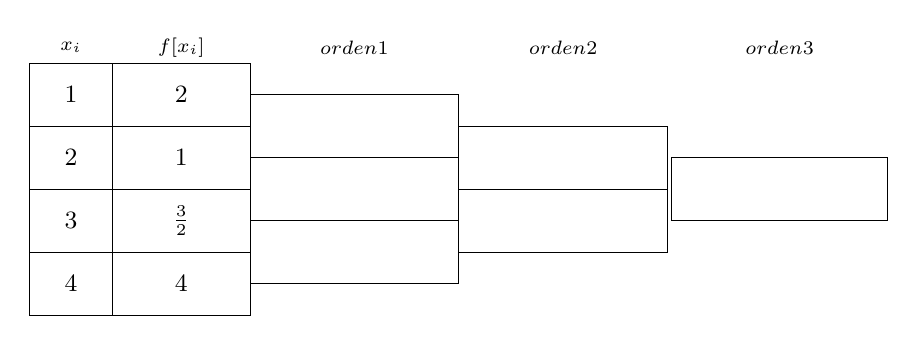
\begin{tikzpicture}[x=1cm,y=1cm]
\path[use as bounding box] (0,-3.65) rectangle (11,-0.0);
\node[font=\scriptsize] at (0.55,-0.25) {$x_i$};
\node[font=\scriptsize] at (1.95,-0.25) {$f[x_i]$};
\node[font=\scriptsize] at (4.15,-0.25) {$\text{orden }1$};
\node[font=\scriptsize] at (6.8,-0.25) {$\text{orden }2$};
\node[font=\scriptsize] at (9.55,-0.25) {$\text{orden }3$};
\node[draw,minimum width=1.05cm,minimum height=.8cm,inner sep=1pt,font=\small] at (0.55,-0.85) {$1$};
\node[draw,minimum width=1.05cm,minimum height=.8cm,inner sep=1pt,font=\small] at (0.55,-1.65) {$2$};
\node[draw,minimum width=1.05cm,minimum height=.8cm,inner sep=1pt,font=\small] at (0.55,-2.45) {$3$};
\node[draw,minimum width=1.05cm,minimum height=.8cm,inner sep=1pt,font=\small] at (0.55,-3.2500000000000004) {$4$};
\node[draw,minimum width=1.75cm,minimum height=.8cm,inner sep=1pt,font=\small] at (1.95,-0.85) {$2$};
\node[draw,minimum width=1.75cm,minimum height=.8cm,inner sep=1pt,font=\small] at (1.95,-1.65) {$1$};
\node[draw,minimum width=1.75cm,minimum height=.8cm,inner sep=1pt,font=\small] at (1.95,-2.45) {$\frac32$};
\node[draw,minimum width=1.75cm,minimum height=.8cm,inner sep=1pt,font=\small] at (1.95,-3.2500000000000004) {$4$};
\node[draw,minimum width=2.65cm,minimum height=.8cm,inner sep=1pt,font=\small] at (4.15,-1.25) {$$};
\node[draw,minimum width=2.65cm,minimum height=.8cm,inner sep=1pt,font=\small] at (4.15,-2.05) {$$};
\node[draw,minimum width=2.65cm,minimum height=.8cm,inner sep=1pt,font=\small] at (4.15,-2.85) {$$};
\node[draw,minimum width=2.65cm,minimum height=.8cm,inner sep=1pt,font=\small] at (6.8,-1.65) {$$};
\node[draw,minimum width=2.65cm,minimum height=.8cm,inner sep=1pt,font=\small] at (6.8,-2.45) {$$};
\node[draw,minimum width=2.75cm,minimum height=.8cm,inner sep=1pt,font=\small] at (9.55,-2.0500000000000003) {$$};
\end{tikzpicture}\end{center}
\small\[f[x_i,\ldots,x_{i+k}]=\frac{f[x_{i+1},\ldots,x_{i+k}]-f[x_i,\ldots,x_{i+k-1}]}{x_{i+k}-x_i}.\]
\end{frame}
\begin{frame}[t]{Diferencias divididas: ejemplo}
\par\noindent\begin{minipage}[t][12mm][t]{\textwidth}\small\strut $f(x)=(x/2)^{x-2}$; nodos $1,2,3,4$; evaluar en $5/2$.\end{minipage}\par\nointerlineskip
\begin{center}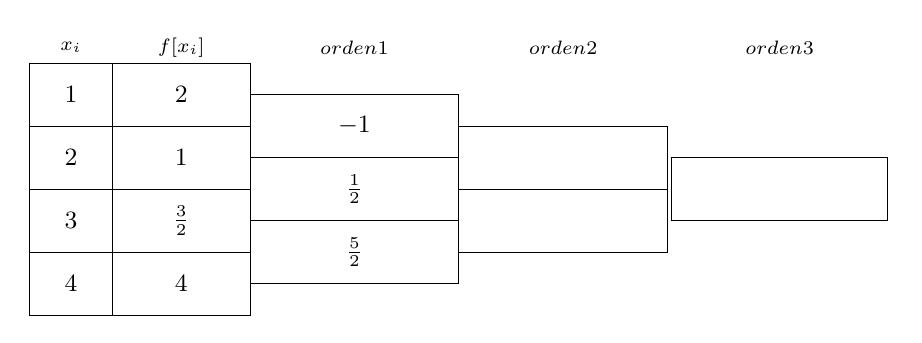
\begin{tikzpicture}[x=1cm,y=1cm]
\path[use as bounding box] (0,-3.65) rectangle (11,-0.0);
\node[font=\scriptsize] at (0.55,-0.25) {$x_i$};
\node[font=\scriptsize] at (1.95,-0.25) {$f[x_i]$};
\node[font=\scriptsize] at (4.15,-0.25) {$\text{orden }1$};
\node[font=\scriptsize] at (6.8,-0.25) {$\text{orden }2$};
\node[font=\scriptsize] at (9.55,-0.25) {$\text{orden }3$};
\node[draw,minimum width=1.05cm,minimum height=.8cm,inner sep=1pt,font=\small] at (0.55,-0.85) {$1$};
\node[draw,minimum width=1.05cm,minimum height=.8cm,inner sep=1pt,font=\small] at (0.55,-1.65) {$2$};
\node[draw,minimum width=1.05cm,minimum height=.8cm,inner sep=1pt,font=\small] at (0.55,-2.45) {$3$};
\node[draw,minimum width=1.05cm,minimum height=.8cm,inner sep=1pt,font=\small] at (0.55,-3.2500000000000004) {$4$};
\node[draw,minimum width=1.75cm,minimum height=.8cm,inner sep=1pt,font=\small] at (1.95,-0.85) {$2$};
\node[draw,minimum width=1.75cm,minimum height=.8cm,inner sep=1pt,font=\small] at (1.95,-1.65) {$1$};
\node[draw,minimum width=1.75cm,minimum height=.8cm,inner sep=1pt,font=\small] at (1.95,-2.45) {$\frac32$};
\node[draw,minimum width=1.75cm,minimum height=.8cm,inner sep=1pt,font=\small] at (1.95,-3.2500000000000004) {$4$};
\node[draw,minimum width=2.65cm,minimum height=.8cm,inner sep=1pt,font=\small] at (4.15,-1.25) {$-1$};
\node[draw,minimum width=2.65cm,minimum height=.8cm,inner sep=1pt,font=\small] at (4.15,-2.05) {$\frac12$};
\node[draw,minimum width=2.65cm,minimum height=.8cm,inner sep=1pt,font=\small] at (4.15,-2.85) {$\frac52$};
\node[draw,minimum width=2.65cm,minimum height=.8cm,inner sep=1pt,font=\small] at (6.8,-1.65) {$$};
\node[draw,minimum width=2.65cm,minimum height=.8cm,inner sep=1pt,font=\small] at (6.8,-2.45) {$$};
\node[draw,minimum width=2.75cm,minimum height=.8cm,inner sep=1pt,font=\small] at (9.55,-2.0500000000000003) {$$};
\end{tikzpicture}\end{center}
\small\[f[1,2]=\frac{1-2}{2-1}=-1,\quad f[2,3]=\frac{3/2-1}{3-2}=\frac12,\quad f[3,4]=\frac{4-3/2}{4-3}=\frac52.\]
\end{frame}
\begin{frame}[t]{Diferencias divididas: ejemplo}
\par\noindent\begin{minipage}[t][12mm][t]{\textwidth}\small\strut $f(x)=(x/2)^{x-2}$; nodos $1,2,3,4$; evaluar en $5/2$.\end{minipage}\par\nointerlineskip
\begin{center}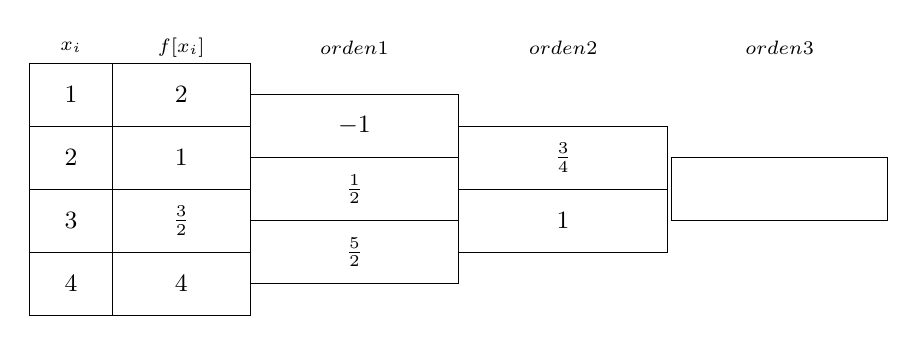
\begin{tikzpicture}[x=1cm,y=1cm]
\path[use as bounding box] (0,-3.65) rectangle (11,-0.0);
\node[font=\scriptsize] at (0.55,-0.25) {$x_i$};
\node[font=\scriptsize] at (1.95,-0.25) {$f[x_i]$};
\node[font=\scriptsize] at (4.15,-0.25) {$\text{orden }1$};
\node[font=\scriptsize] at (6.8,-0.25) {$\text{orden }2$};
\node[font=\scriptsize] at (9.55,-0.25) {$\text{orden }3$};
\node[draw,minimum width=1.05cm,minimum height=.8cm,inner sep=1pt,font=\small] at (0.55,-0.85) {$1$};
\node[draw,minimum width=1.05cm,minimum height=.8cm,inner sep=1pt,font=\small] at (0.55,-1.65) {$2$};
\node[draw,minimum width=1.05cm,minimum height=.8cm,inner sep=1pt,font=\small] at (0.55,-2.45) {$3$};
\node[draw,minimum width=1.05cm,minimum height=.8cm,inner sep=1pt,font=\small] at (0.55,-3.2500000000000004) {$4$};
\node[draw,minimum width=1.75cm,minimum height=.8cm,inner sep=1pt,font=\small] at (1.95,-0.85) {$2$};
\node[draw,minimum width=1.75cm,minimum height=.8cm,inner sep=1pt,font=\small] at (1.95,-1.65) {$1$};
\node[draw,minimum width=1.75cm,minimum height=.8cm,inner sep=1pt,font=\small] at (1.95,-2.45) {$\frac32$};
\node[draw,minimum width=1.75cm,minimum height=.8cm,inner sep=1pt,font=\small] at (1.95,-3.2500000000000004) {$4$};
\node[draw,minimum width=2.65cm,minimum height=.8cm,inner sep=1pt,font=\small] at (4.15,-1.25) {$-1$};
\node[draw,minimum width=2.65cm,minimum height=.8cm,inner sep=1pt,font=\small] at (4.15,-2.05) {$\frac12$};
\node[draw,minimum width=2.65cm,minimum height=.8cm,inner sep=1pt,font=\small] at (4.15,-2.85) {$\frac52$};
\node[draw,minimum width=2.65cm,minimum height=.8cm,inner sep=1pt,font=\small] at (6.8,-1.65) {$\frac34$};
\node[draw,minimum width=2.65cm,minimum height=.8cm,inner sep=1pt,font=\small] at (6.8,-2.45) {$1$};
\node[draw,minimum width=2.75cm,minimum height=.8cm,inner sep=1pt,font=\small] at (9.55,-2.0500000000000003) {$$};
\end{tikzpicture}\end{center}
\small\[f[1,2,3]=\frac{1/2-(-1)}{3-1}=\frac34,\quad f[2,3,4]=\frac{5/2-1/2}{4-2}=1.\]
\end{frame}
\begin{frame}[t]{Diferencias divididas: ejemplo}
\par\noindent\begin{minipage}[t][12mm][t]{\textwidth}\small\strut $f(x)=(x/2)^{x-2}$; nodos $1,2,3,4$; evaluar en $5/2$.\end{minipage}\par\nointerlineskip
\begin{center}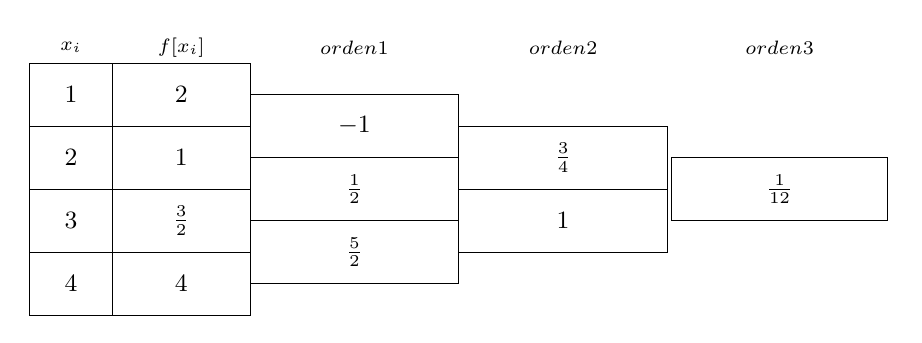
\begin{tikzpicture}[x=1cm,y=1cm]
\path[use as bounding box] (0,-3.65) rectangle (11,-0.0);
\node[font=\scriptsize] at (0.55,-0.25) {$x_i$};
\node[font=\scriptsize] at (1.95,-0.25) {$f[x_i]$};
\node[font=\scriptsize] at (4.15,-0.25) {$\text{orden }1$};
\node[font=\scriptsize] at (6.8,-0.25) {$\text{orden }2$};
\node[font=\scriptsize] at (9.55,-0.25) {$\text{orden }3$};
\node[draw,minimum width=1.05cm,minimum height=.8cm,inner sep=1pt,font=\small] at (0.55,-0.85) {$1$};
\node[draw,minimum width=1.05cm,minimum height=.8cm,inner sep=1pt,font=\small] at (0.55,-1.65) {$2$};
\node[draw,minimum width=1.05cm,minimum height=.8cm,inner sep=1pt,font=\small] at (0.55,-2.45) {$3$};
\node[draw,minimum width=1.05cm,minimum height=.8cm,inner sep=1pt,font=\small] at (0.55,-3.2500000000000004) {$4$};
\node[draw,minimum width=1.75cm,minimum height=.8cm,inner sep=1pt,font=\small] at (1.95,-0.85) {$2$};
\node[draw,minimum width=1.75cm,minimum height=.8cm,inner sep=1pt,font=\small] at (1.95,-1.65) {$1$};
\node[draw,minimum width=1.75cm,minimum height=.8cm,inner sep=1pt,font=\small] at (1.95,-2.45) {$\frac32$};
\node[draw,minimum width=1.75cm,minimum height=.8cm,inner sep=1pt,font=\small] at (1.95,-3.2500000000000004) {$4$};
\node[draw,minimum width=2.65cm,minimum height=.8cm,inner sep=1pt,font=\small] at (4.15,-1.25) {$-1$};
\node[draw,minimum width=2.65cm,minimum height=.8cm,inner sep=1pt,font=\small] at (4.15,-2.05) {$\frac12$};
\node[draw,minimum width=2.65cm,minimum height=.8cm,inner sep=1pt,font=\small] at (4.15,-2.85) {$\frac52$};
\node[draw,minimum width=2.65cm,minimum height=.8cm,inner sep=1pt,font=\small] at (6.8,-1.65) {$\frac34$};
\node[draw,minimum width=2.65cm,minimum height=.8cm,inner sep=1pt,font=\small] at (6.8,-2.45) {$1$};
\node[draw,minimum width=2.75cm,minimum height=.8cm,inner sep=1pt,font=\small] at (9.55,-2.0500000000000003) {$\frac1{12}$};
\end{tikzpicture}\end{center}
\small\[f[1,2,3,4]=\frac{1-3/4}{4-1}=\frac1{12}.\]
\end{frame}
\begin{frame}[t]{Newton: polinomio lineal}
\par\noindent\begin{minipage}[t][12mm][t]{\textwidth}\small\strut $f(x)=(x/2)^{x-2}$; nodos $1,2,3,4$; evaluar en $5/2$.\end{minipage}\par\nointerlineskip
\begin{center}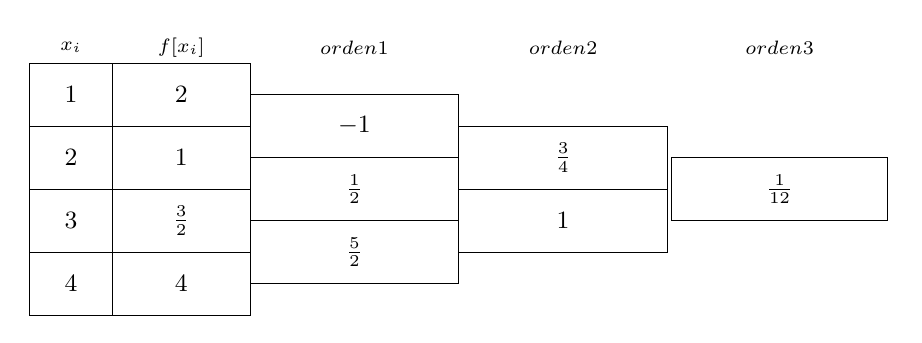
\begin{tikzpicture}[x=1cm,y=1cm]
\path[use as bounding box] (0,-3.65) rectangle (11,-0.0);
\node[font=\scriptsize] at (0.55,-0.25) {$x_i$};
\node[font=\scriptsize] at (1.95,-0.25) {$f[x_i]$};
\node[font=\scriptsize] at (4.15,-0.25) {$\text{orden }1$};
\node[font=\scriptsize] at (6.8,-0.25) {$\text{orden }2$};
\node[font=\scriptsize] at (9.55,-0.25) {$\text{orden }3$};
\node[draw,minimum width=1.05cm,minimum height=.8cm,inner sep=1pt,font=\small] at (0.55,-0.85) {$1$};
\node[draw,minimum width=1.05cm,minimum height=.8cm,inner sep=1pt,font=\small] at (0.55,-1.65) {$2$};
\node[draw,minimum width=1.05cm,minimum height=.8cm,inner sep=1pt,font=\small] at (0.55,-2.45) {$3$};
\node[draw,minimum width=1.05cm,minimum height=.8cm,inner sep=1pt,font=\small] at (0.55,-3.2500000000000004) {$4$};
\node[draw,minimum width=1.75cm,minimum height=.8cm,inner sep=1pt,font=\small] at (1.95,-0.85) {$2$};
\node[draw,minimum width=1.75cm,minimum height=.8cm,inner sep=1pt,font=\small] at (1.95,-1.65) {$1$};
\node[draw,minimum width=1.75cm,minimum height=.8cm,inner sep=1pt,font=\small] at (1.95,-2.45) {$\frac32$};
\node[draw,minimum width=1.75cm,minimum height=.8cm,inner sep=1pt,font=\small] at (1.95,-3.2500000000000004) {$4$};
\node[draw,minimum width=2.65cm,minimum height=.8cm,inner sep=1pt,font=\small] at (4.15,-1.25) {$-1$};
\node[draw,minimum width=2.65cm,minimum height=.8cm,inner sep=1pt,font=\small] at (4.15,-2.05) {$\frac12$};
\node[draw,minimum width=2.65cm,minimum height=.8cm,inner sep=1pt,font=\small] at (4.15,-2.85) {$\frac52$};
\node[draw,minimum width=2.65cm,minimum height=.8cm,inner sep=1pt,font=\small] at (6.8,-1.65) {$\frac34$};
\node[draw,minimum width=2.65cm,minimum height=.8cm,inner sep=1pt,font=\small] at (6.8,-2.45) {$1$};
\node[draw,minimum width=2.75cm,minimum height=.8cm,inner sep=1pt,font=\small] at (9.55,-2.0500000000000003) {$\frac1{12}$};
\end{tikzpicture}\end{center}
\[P_1(x)=2-(x-1),\qquad P_1(5/2)=1/2.\]
\end{frame}
\begin{frame}[t]{Newton: polinomio cuadrático}
\par\noindent\begin{minipage}[t][12mm][t]{\textwidth}\small\strut $f(x)=(x/2)^{x-2}$; nodos $1,2,3,4$; evaluar en $5/2$.\end{minipage}\par\nointerlineskip
\begin{center}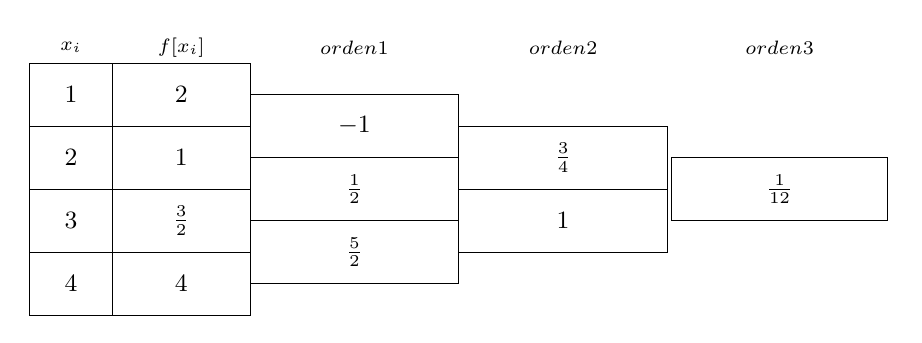
\begin{tikzpicture}[x=1cm,y=1cm]
\path[use as bounding box] (0,-3.65) rectangle (11,-0.0);
\node[font=\scriptsize] at (0.55,-0.25) {$x_i$};
\node[font=\scriptsize] at (1.95,-0.25) {$f[x_i]$};
\node[font=\scriptsize] at (4.15,-0.25) {$\text{orden }1$};
\node[font=\scriptsize] at (6.8,-0.25) {$\text{orden }2$};
\node[font=\scriptsize] at (9.55,-0.25) {$\text{orden }3$};
\node[draw,minimum width=1.05cm,minimum height=.8cm,inner sep=1pt,font=\small] at (0.55,-0.85) {$1$};
\node[draw,minimum width=1.05cm,minimum height=.8cm,inner sep=1pt,font=\small] at (0.55,-1.65) {$2$};
\node[draw,minimum width=1.05cm,minimum height=.8cm,inner sep=1pt,font=\small] at (0.55,-2.45) {$3$};
\node[draw,minimum width=1.05cm,minimum height=.8cm,inner sep=1pt,font=\small] at (0.55,-3.2500000000000004) {$4$};
\node[draw,minimum width=1.75cm,minimum height=.8cm,inner sep=1pt,font=\small] at (1.95,-0.85) {$2$};
\node[draw,minimum width=1.75cm,minimum height=.8cm,inner sep=1pt,font=\small] at (1.95,-1.65) {$1$};
\node[draw,minimum width=1.75cm,minimum height=.8cm,inner sep=1pt,font=\small] at (1.95,-2.45) {$\frac32$};
\node[draw,minimum width=1.75cm,minimum height=.8cm,inner sep=1pt,font=\small] at (1.95,-3.2500000000000004) {$4$};
\node[draw,minimum width=2.65cm,minimum height=.8cm,inner sep=1pt,font=\small] at (4.15,-1.25) {$-1$};
\node[draw,minimum width=2.65cm,minimum height=.8cm,inner sep=1pt,font=\small] at (4.15,-2.05) {$\frac12$};
\node[draw,minimum width=2.65cm,minimum height=.8cm,inner sep=1pt,font=\small] at (4.15,-2.85) {$\frac52$};
\node[draw,minimum width=2.65cm,minimum height=.8cm,inner sep=1pt,font=\small] at (6.8,-1.65) {$\frac34$};
\node[draw,minimum width=2.65cm,minimum height=.8cm,inner sep=1pt,font=\small] at (6.8,-2.45) {$1$};
\node[draw,minimum width=2.75cm,minimum height=.8cm,inner sep=1pt,font=\small] at (9.55,-2.0500000000000003) {$\frac1{12}$};
\end{tikzpicture}\end{center}
\small
\[P_2(x)=P_1(x)+\tfrac34(x-1)(x-2).\]
\[P_2(5/2)=\tfrac12+\tfrac34\cdot\tfrac32\cdot\tfrac12=\tfrac{17}{16}.\]
\end{frame}
\begin{frame}[t]{Newton: polinomio cúbico}
\par\noindent\begin{minipage}[t][12mm][t]{\textwidth}\small\strut $f(x)=(x/2)^{x-2}$; nodos $1,2,3,4$; evaluar en $5/2$.\end{minipage}\par\nointerlineskip
\begin{center}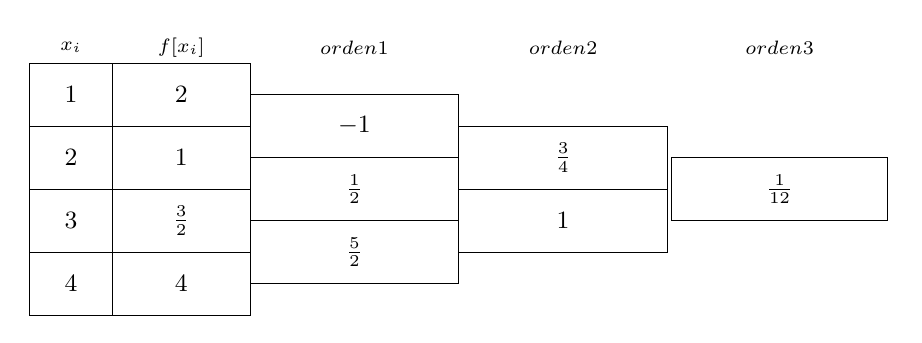
\begin{tikzpicture}[x=1cm,y=1cm]
\path[use as bounding box] (0,-3.65) rectangle (11,-0.0);
\node[font=\scriptsize] at (0.55,-0.25) {$x_i$};
\node[font=\scriptsize] at (1.95,-0.25) {$f[x_i]$};
\node[font=\scriptsize] at (4.15,-0.25) {$\text{orden }1$};
\node[font=\scriptsize] at (6.8,-0.25) {$\text{orden }2$};
\node[font=\scriptsize] at (9.55,-0.25) {$\text{orden }3$};
\node[draw,minimum width=1.05cm,minimum height=.8cm,inner sep=1pt,font=\small] at (0.55,-0.85) {$1$};
\node[draw,minimum width=1.05cm,minimum height=.8cm,inner sep=1pt,font=\small] at (0.55,-1.65) {$2$};
\node[draw,minimum width=1.05cm,minimum height=.8cm,inner sep=1pt,font=\small] at (0.55,-2.45) {$3$};
\node[draw,minimum width=1.05cm,minimum height=.8cm,inner sep=1pt,font=\small] at (0.55,-3.2500000000000004) {$4$};
\node[draw,minimum width=1.75cm,minimum height=.8cm,inner sep=1pt,font=\small] at (1.95,-0.85) {$2$};
\node[draw,minimum width=1.75cm,minimum height=.8cm,inner sep=1pt,font=\small] at (1.95,-1.65) {$1$};
\node[draw,minimum width=1.75cm,minimum height=.8cm,inner sep=1pt,font=\small] at (1.95,-2.45) {$\frac32$};
\node[draw,minimum width=1.75cm,minimum height=.8cm,inner sep=1pt,font=\small] at (1.95,-3.2500000000000004) {$4$};
\node[draw,minimum width=2.65cm,minimum height=.8cm,inner sep=1pt,font=\small] at (4.15,-1.25) {$-1$};
\node[draw,minimum width=2.65cm,minimum height=.8cm,inner sep=1pt,font=\small] at (4.15,-2.05) {$\frac12$};
\node[draw,minimum width=2.65cm,minimum height=.8cm,inner sep=1pt,font=\small] at (4.15,-2.85) {$\frac52$};
\node[draw,minimum width=2.65cm,minimum height=.8cm,inner sep=1pt,font=\small] at (6.8,-1.65) {$\frac34$};
\node[draw,minimum width=2.65cm,minimum height=.8cm,inner sep=1pt,font=\small] at (6.8,-2.45) {$1$};
\node[draw,minimum width=2.75cm,minimum height=.8cm,inner sep=1pt,font=\small] at (9.55,-2.0500000000000003) {$\frac1{12}$};
\end{tikzpicture}\end{center}
\small
\[P_3(x)=P_2(x)+\tfrac1{12}(x-1)(x-2)(x-3).\]
\[P_3(5/2)=\tfrac{17}{16}-\tfrac1{32}=\tfrac{33}{32}.\]
\end{frame}
\begin{frame}[t]{Diferencias divididas: otro ejemplo}
\par\noindent\begin{minipage}[t][12mm][t]{\textwidth}\small\strut Obtener el polinomio interpolante de los datos dados.\end{minipage}\par\nointerlineskip
\begingroup\small\setlength{\tabcolsep}{3pt}\begin{center}\begin{tabular}{|C{.2\textwidth}|C{.2\textwidth}|}\hline
\rule[-2mm]{0pt}{6mm}$x$&$f(x)$\\\hline
\rule[-2.5mm]{0pt}{7mm}$-1$&$15$\\\hline
\rule[-2.5mm]{0pt}{7mm}$0$&$8$\\\hline
\rule[-2.5mm]{0pt}{7mm}$3$&$-1$\\\hline
\end{tabular}\end{center}\endgroup\par

\end{frame}
\begin{frame}[t]{Diferencias divididas: otro ejemplo}
\par\noindent\begin{minipage}[t][12mm][t]{\textwidth}\small\strut Obtener el polinomio interpolante de los datos dados.\end{minipage}\par\nointerlineskip
\begin{center}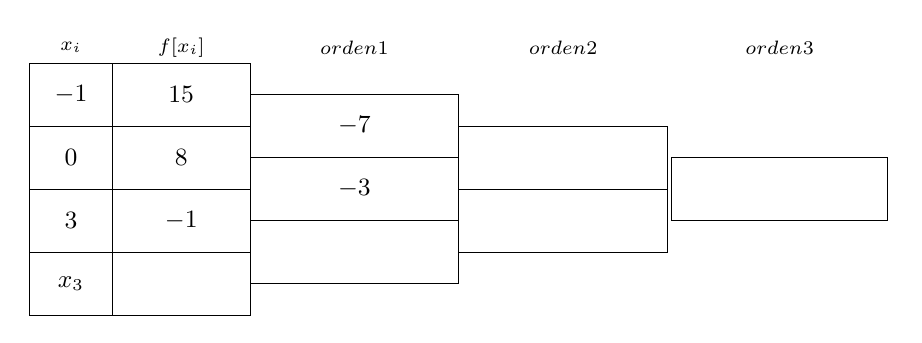
\begin{tikzpicture}[x=1cm,y=1cm]
\path[use as bounding box] (0,-3.65) rectangle (11,-0.0);
\node[font=\scriptsize] at (0.55,-0.25) {$x_i$};
\node[font=\scriptsize] at (1.95,-0.25) {$f[x_i]$};
\node[font=\scriptsize] at (4.15,-0.25) {$\text{orden }1$};
\node[font=\scriptsize] at (6.8,-0.25) {$\text{orden }2$};
\node[font=\scriptsize] at (9.55,-0.25) {$\text{orden }3$};
\node[draw,minimum width=1.05cm,minimum height=.8cm,inner sep=1pt,font=\small] at (0.55,-0.85) {$-1$};
\node[draw,minimum width=1.05cm,minimum height=.8cm,inner sep=1pt,font=\small] at (0.55,-1.65) {$0$};
\node[draw,minimum width=1.05cm,minimum height=.8cm,inner sep=1pt,font=\small] at (0.55,-2.45) {$3$};
\node[draw,minimum width=1.05cm,minimum height=.8cm,inner sep=1pt,font=\small] at (0.55,-3.2500000000000004) {$x_3$};
\node[draw,minimum width=1.75cm,minimum height=.8cm,inner sep=1pt,font=\small] at (1.95,-0.85) {$15$};
\node[draw,minimum width=1.75cm,minimum height=.8cm,inner sep=1pt,font=\small] at (1.95,-1.65) {$8$};
\node[draw,minimum width=1.75cm,minimum height=.8cm,inner sep=1pt,font=\small] at (1.95,-2.45) {$-1$};
\node[draw,minimum width=1.75cm,minimum height=.8cm,inner sep=1pt,font=\small] at (1.95,-3.2500000000000004) {$$};
\node[draw,minimum width=2.65cm,minimum height=.8cm,inner sep=1pt,font=\small] at (4.15,-1.25) {$-7$};
\node[draw,minimum width=2.65cm,minimum height=.8cm,inner sep=1pt,font=\small] at (4.15,-2.05) {$-3$};
\node[draw,minimum width=2.65cm,minimum height=.8cm,inner sep=1pt,font=\small] at (4.15,-2.85) {$$};
\node[draw,minimum width=2.65cm,minimum height=.8cm,inner sep=1pt,font=\small] at (6.8,-1.65) {$$};
\node[draw,minimum width=2.65cm,minimum height=.8cm,inner sep=1pt,font=\small] at (6.8,-2.45) {$$};
\node[draw,minimum width=2.75cm,minimum height=.8cm,inner sep=1pt,font=\small] at (9.55,-2.0500000000000003) {$$};
\end{tikzpicture}\end{center}
\small\[f[-1,0]=\frac{8-15}{0+1}=-7,\qquad f[0,3]=\frac{-1-8}{3-0}=-3.\]
\end{frame}
\begin{frame}[t]{Diferencias divididas: otro ejemplo}
\par\noindent\begin{minipage}[t][12mm][t]{\textwidth}\small\strut Obtener el polinomio interpolante de los datos dados.\end{minipage}\par\nointerlineskip
\begin{center}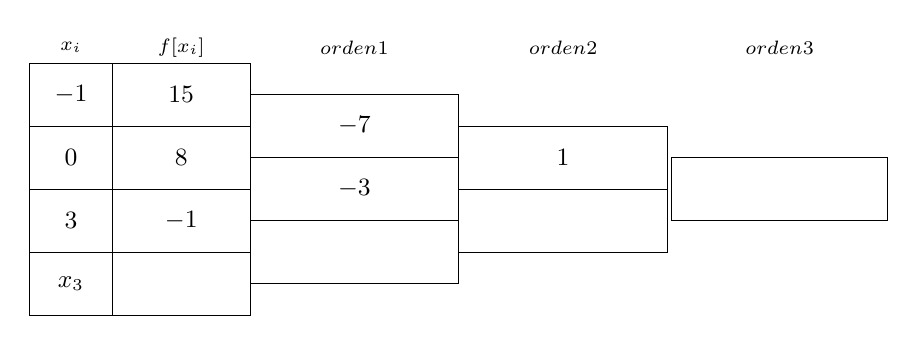
\begin{tikzpicture}[x=1cm,y=1cm]
\path[use as bounding box] (0,-3.65) rectangle (11,-0.0);
\node[font=\scriptsize] at (0.55,-0.25) {$x_i$};
\node[font=\scriptsize] at (1.95,-0.25) {$f[x_i]$};
\node[font=\scriptsize] at (4.15,-0.25) {$\text{orden }1$};
\node[font=\scriptsize] at (6.8,-0.25) {$\text{orden }2$};
\node[font=\scriptsize] at (9.55,-0.25) {$\text{orden }3$};
\node[draw,minimum width=1.05cm,minimum height=.8cm,inner sep=1pt,font=\small] at (0.55,-0.85) {$-1$};
\node[draw,minimum width=1.05cm,minimum height=.8cm,inner sep=1pt,font=\small] at (0.55,-1.65) {$0$};
\node[draw,minimum width=1.05cm,minimum height=.8cm,inner sep=1pt,font=\small] at (0.55,-2.45) {$3$};
\node[draw,minimum width=1.05cm,minimum height=.8cm,inner sep=1pt,font=\small] at (0.55,-3.2500000000000004) {$x_3$};
\node[draw,minimum width=1.75cm,minimum height=.8cm,inner sep=1pt,font=\small] at (1.95,-0.85) {$15$};
\node[draw,minimum width=1.75cm,minimum height=.8cm,inner sep=1pt,font=\small] at (1.95,-1.65) {$8$};
\node[draw,minimum width=1.75cm,minimum height=.8cm,inner sep=1pt,font=\small] at (1.95,-2.45) {$-1$};
\node[draw,minimum width=1.75cm,minimum height=.8cm,inner sep=1pt,font=\small] at (1.95,-3.2500000000000004) {$$};
\node[draw,minimum width=2.65cm,minimum height=.8cm,inner sep=1pt,font=\small] at (4.15,-1.25) {$-7$};
\node[draw,minimum width=2.65cm,minimum height=.8cm,inner sep=1pt,font=\small] at (4.15,-2.05) {$-3$};
\node[draw,minimum width=2.65cm,minimum height=.8cm,inner sep=1pt,font=\small] at (4.15,-2.85) {$$};
\node[draw,minimum width=2.65cm,minimum height=.8cm,inner sep=1pt,font=\small] at (6.8,-1.65) {$1$};
\node[draw,minimum width=2.65cm,minimum height=.8cm,inner sep=1pt,font=\small] at (6.8,-2.45) {$$};
\node[draw,minimum width=2.75cm,minimum height=.8cm,inner sep=1pt,font=\small] at (9.55,-2.0500000000000003) {$$};
\end{tikzpicture}\end{center}
\small\[f[-1,0,3]=\frac{-3-(-7)}{3-(-1)}=1.\]
\end{frame}
\begin{frame}[t]{Diferencias divididas: otro ejemplo}
\par\noindent\begin{minipage}[t][12mm][t]{\textwidth}\small\strut Obtener el polinomio interpolante de los datos dados.\end{minipage}\par\nointerlineskip
\begin{center}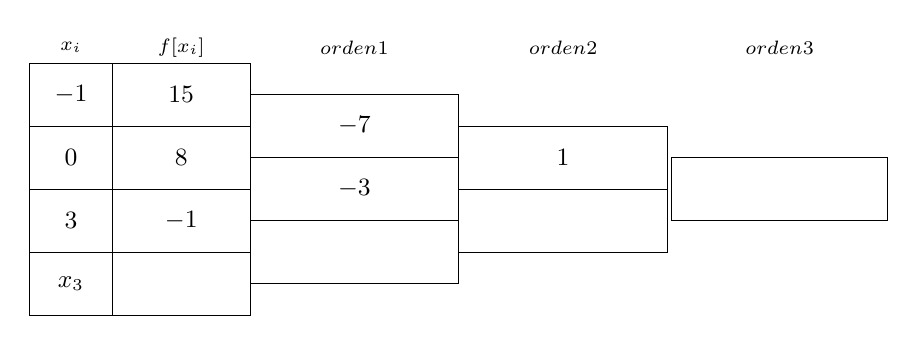
\begin{tikzpicture}[x=1cm,y=1cm]
\path[use as bounding box] (0,-3.65) rectangle (11,-0.0);
\node[font=\scriptsize] at (0.55,-0.25) {$x_i$};
\node[font=\scriptsize] at (1.95,-0.25) {$f[x_i]$};
\node[font=\scriptsize] at (4.15,-0.25) {$\text{orden }1$};
\node[font=\scriptsize] at (6.8,-0.25) {$\text{orden }2$};
\node[font=\scriptsize] at (9.55,-0.25) {$\text{orden }3$};
\node[draw,minimum width=1.05cm,minimum height=.8cm,inner sep=1pt,font=\small] at (0.55,-0.85) {$-1$};
\node[draw,minimum width=1.05cm,minimum height=.8cm,inner sep=1pt,font=\small] at (0.55,-1.65) {$0$};
\node[draw,minimum width=1.05cm,minimum height=.8cm,inner sep=1pt,font=\small] at (0.55,-2.45) {$3$};
\node[draw,minimum width=1.05cm,minimum height=.8cm,inner sep=1pt,font=\small] at (0.55,-3.2500000000000004) {$x_3$};
\node[draw,minimum width=1.75cm,minimum height=.8cm,inner sep=1pt,font=\small] at (1.95,-0.85) {$15$};
\node[draw,minimum width=1.75cm,minimum height=.8cm,inner sep=1pt,font=\small] at (1.95,-1.65) {$8$};
\node[draw,minimum width=1.75cm,minimum height=.8cm,inner sep=1pt,font=\small] at (1.95,-2.45) {$-1$};
\node[draw,minimum width=1.75cm,minimum height=.8cm,inner sep=1pt,font=\small] at (1.95,-3.2500000000000004) {$$};
\node[draw,minimum width=2.65cm,minimum height=.8cm,inner sep=1pt,font=\small] at (4.15,-1.25) {$-7$};
\node[draw,minimum width=2.65cm,minimum height=.8cm,inner sep=1pt,font=\small] at (4.15,-2.05) {$-3$};
\node[draw,minimum width=2.65cm,minimum height=.8cm,inner sep=1pt,font=\small] at (4.15,-2.85) {$$};
\node[draw,minimum width=2.65cm,minimum height=.8cm,inner sep=1pt,font=\small] at (6.8,-1.65) {$1$};
\node[draw,minimum width=2.65cm,minimum height=.8cm,inner sep=1pt,font=\small] at (6.8,-2.45) {$$};
\node[draw,minimum width=2.75cm,minimum height=.8cm,inner sep=1pt,font=\small] at (9.55,-2.0500000000000003) {$$};
\end{tikzpicture}\end{center}
\small\[P_2(x)=15-7(x+1)+(x+1)x=x^2-6x+8.\]
\end{frame}
\begin{frame}[t]{Diferencias divididas: ampliación}
\par\noindent\begin{minipage}[t][12mm][t]{\textwidth}\small\strut Ampliar el polinomio con el nuevo dato $x_3=5$, $f(5)=-5$.\end{minipage}\par\nointerlineskip
\begin{center}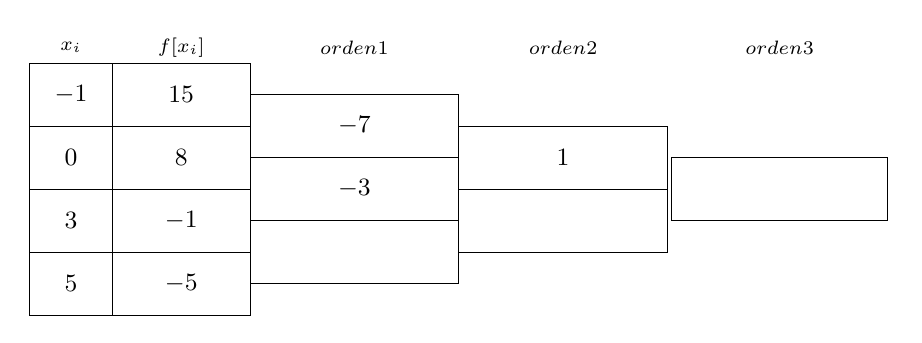
\begin{tikzpicture}[x=1cm,y=1cm]
\path[use as bounding box] (0,-3.65) rectangle (11,-0.0);
\node[font=\scriptsize] at (0.55,-0.25) {$x_i$};
\node[font=\scriptsize] at (1.95,-0.25) {$f[x_i]$};
\node[font=\scriptsize] at (4.15,-0.25) {$\text{orden }1$};
\node[font=\scriptsize] at (6.8,-0.25) {$\text{orden }2$};
\node[font=\scriptsize] at (9.55,-0.25) {$\text{orden }3$};
\node[draw,minimum width=1.05cm,minimum height=.8cm,inner sep=1pt,font=\small] at (0.55,-0.85) {$-1$};
\node[draw,minimum width=1.05cm,minimum height=.8cm,inner sep=1pt,font=\small] at (0.55,-1.65) {$0$};
\node[draw,minimum width=1.05cm,minimum height=.8cm,inner sep=1pt,font=\small] at (0.55,-2.45) {$3$};
\node[draw,minimum width=1.05cm,minimum height=.8cm,inner sep=1pt,font=\small] at (0.55,-3.2500000000000004) {$5$};
\node[draw,minimum width=1.75cm,minimum height=.8cm,inner sep=1pt,font=\small] at (1.95,-0.85) {$15$};
\node[draw,minimum width=1.75cm,minimum height=.8cm,inner sep=1pt,font=\small] at (1.95,-1.65) {$8$};
\node[draw,minimum width=1.75cm,minimum height=.8cm,inner sep=1pt,font=\small] at (1.95,-2.45) {$-1$};
\node[draw,minimum width=1.75cm,minimum height=.8cm,inner sep=1pt,font=\small] at (1.95,-3.2500000000000004) {$-5$};
\node[draw,minimum width=2.65cm,minimum height=.8cm,inner sep=1pt,font=\small] at (4.15,-1.25) {$-7$};
\node[draw,minimum width=2.65cm,minimum height=.8cm,inner sep=1pt,font=\small] at (4.15,-2.05) {$-3$};
\node[draw,minimum width=2.65cm,minimum height=.8cm,inner sep=1pt,font=\small] at (4.15,-2.85) {$$};
\node[draw,minimum width=2.65cm,minimum height=.8cm,inner sep=1pt,font=\small] at (6.8,-1.65) {$1$};
\node[draw,minimum width=2.65cm,minimum height=.8cm,inner sep=1pt,font=\small] at (6.8,-2.45) {$$};
\node[draw,minimum width=2.75cm,minimum height=.8cm,inner sep=1pt,font=\small] at (9.55,-2.0500000000000003) {$$};
\end{tikzpicture}\end{center}
\[P_2(x)=x^2-6x+8.\]
\end{frame}
\begin{frame}[t]{Diferencias divididas: ampliación}
\par\noindent\begin{minipage}[t][12mm][t]{\textwidth}\small\strut Ampliar el polinomio con el nuevo dato $x_3=5$, $f(5)=-5$.\end{minipage}\par\nointerlineskip
\begin{center}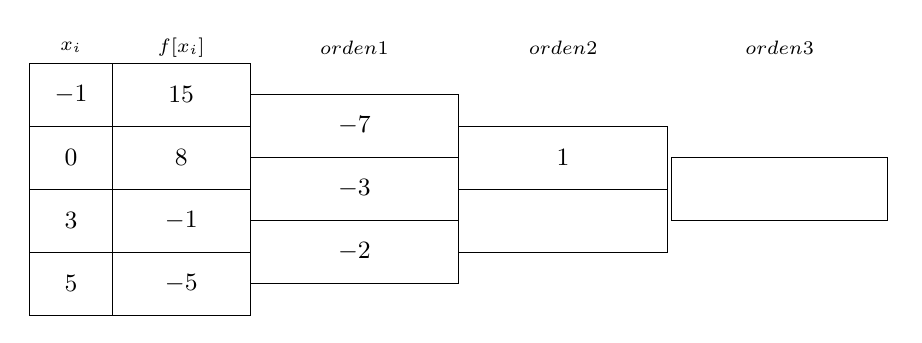
\begin{tikzpicture}[x=1cm,y=1cm]
\path[use as bounding box] (0,-3.65) rectangle (11,-0.0);
\node[font=\scriptsize] at (0.55,-0.25) {$x_i$};
\node[font=\scriptsize] at (1.95,-0.25) {$f[x_i]$};
\node[font=\scriptsize] at (4.15,-0.25) {$\text{orden }1$};
\node[font=\scriptsize] at (6.8,-0.25) {$\text{orden }2$};
\node[font=\scriptsize] at (9.55,-0.25) {$\text{orden }3$};
\node[draw,minimum width=1.05cm,minimum height=.8cm,inner sep=1pt,font=\small] at (0.55,-0.85) {$-1$};
\node[draw,minimum width=1.05cm,minimum height=.8cm,inner sep=1pt,font=\small] at (0.55,-1.65) {$0$};
\node[draw,minimum width=1.05cm,minimum height=.8cm,inner sep=1pt,font=\small] at (0.55,-2.45) {$3$};
\node[draw,minimum width=1.05cm,minimum height=.8cm,inner sep=1pt,font=\small] at (0.55,-3.2500000000000004) {$5$};
\node[draw,minimum width=1.75cm,minimum height=.8cm,inner sep=1pt,font=\small] at (1.95,-0.85) {$15$};
\node[draw,minimum width=1.75cm,minimum height=.8cm,inner sep=1pt,font=\small] at (1.95,-1.65) {$8$};
\node[draw,minimum width=1.75cm,minimum height=.8cm,inner sep=1pt,font=\small] at (1.95,-2.45) {$-1$};
\node[draw,minimum width=1.75cm,minimum height=.8cm,inner sep=1pt,font=\small] at (1.95,-3.2500000000000004) {$-5$};
\node[draw,minimum width=2.65cm,minimum height=.8cm,inner sep=1pt,font=\small] at (4.15,-1.25) {$-7$};
\node[draw,minimum width=2.65cm,minimum height=.8cm,inner sep=1pt,font=\small] at (4.15,-2.05) {$-3$};
\node[draw,minimum width=2.65cm,minimum height=.8cm,inner sep=1pt,font=\small] at (4.15,-2.85) {$-2$};
\node[draw,minimum width=2.65cm,minimum height=.8cm,inner sep=1pt,font=\small] at (6.8,-1.65) {$1$};
\node[draw,minimum width=2.65cm,minimum height=.8cm,inner sep=1pt,font=\small] at (6.8,-2.45) {$$};
\node[draw,minimum width=2.75cm,minimum height=.8cm,inner sep=1pt,font=\small] at (9.55,-2.0500000000000003) {$$};
\end{tikzpicture}\end{center}
\[f[3,5]=\frac{-5-(-1)}{5-3}=-2.\]
\end{frame}
\begin{frame}[t]{Diferencias divididas: ampliación}
\par\noindent\begin{minipage}[t][12mm][t]{\textwidth}\small\strut Ampliar el polinomio con el nuevo dato $x_3=5$, $f(5)=-5$.\end{minipage}\par\nointerlineskip
\begin{center}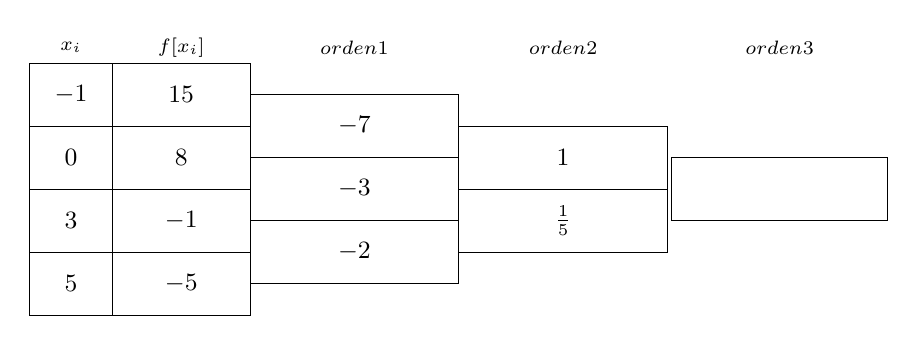
\begin{tikzpicture}[x=1cm,y=1cm]
\path[use as bounding box] (0,-3.65) rectangle (11,-0.0);
\node[font=\scriptsize] at (0.55,-0.25) {$x_i$};
\node[font=\scriptsize] at (1.95,-0.25) {$f[x_i]$};
\node[font=\scriptsize] at (4.15,-0.25) {$\text{orden }1$};
\node[font=\scriptsize] at (6.8,-0.25) {$\text{orden }2$};
\node[font=\scriptsize] at (9.55,-0.25) {$\text{orden }3$};
\node[draw,minimum width=1.05cm,minimum height=.8cm,inner sep=1pt,font=\small] at (0.55,-0.85) {$-1$};
\node[draw,minimum width=1.05cm,minimum height=.8cm,inner sep=1pt,font=\small] at (0.55,-1.65) {$0$};
\node[draw,minimum width=1.05cm,minimum height=.8cm,inner sep=1pt,font=\small] at (0.55,-2.45) {$3$};
\node[draw,minimum width=1.05cm,minimum height=.8cm,inner sep=1pt,font=\small] at (0.55,-3.2500000000000004) {$5$};
\node[draw,minimum width=1.75cm,minimum height=.8cm,inner sep=1pt,font=\small] at (1.95,-0.85) {$15$};
\node[draw,minimum width=1.75cm,minimum height=.8cm,inner sep=1pt,font=\small] at (1.95,-1.65) {$8$};
\node[draw,minimum width=1.75cm,minimum height=.8cm,inner sep=1pt,font=\small] at (1.95,-2.45) {$-1$};
\node[draw,minimum width=1.75cm,minimum height=.8cm,inner sep=1pt,font=\small] at (1.95,-3.2500000000000004) {$-5$};
\node[draw,minimum width=2.65cm,minimum height=.8cm,inner sep=1pt,font=\small] at (4.15,-1.25) {$-7$};
\node[draw,minimum width=2.65cm,minimum height=.8cm,inner sep=1pt,font=\small] at (4.15,-2.05) {$-3$};
\node[draw,minimum width=2.65cm,minimum height=.8cm,inner sep=1pt,font=\small] at (4.15,-2.85) {$-2$};
\node[draw,minimum width=2.65cm,minimum height=.8cm,inner sep=1pt,font=\small] at (6.8,-1.65) {$1$};
\node[draw,minimum width=2.65cm,minimum height=.8cm,inner sep=1pt,font=\small] at (6.8,-2.45) {$\frac15$};
\node[draw,minimum width=2.75cm,minimum height=.8cm,inner sep=1pt,font=\small] at (9.55,-2.0500000000000003) {$$};
\end{tikzpicture}\end{center}
\[f[0,3,5]=\frac{-2-(-3)}{5-0}=\frac15.\]
\end{frame}
\begin{frame}[t]{Diferencias divididas: ampliación}
\par\noindent\begin{minipage}[t][12mm][t]{\textwidth}\small\strut Ampliar el polinomio con el nuevo dato $x_3=5$, $f(5)=-5$.\end{minipage}\par\nointerlineskip
\begin{center}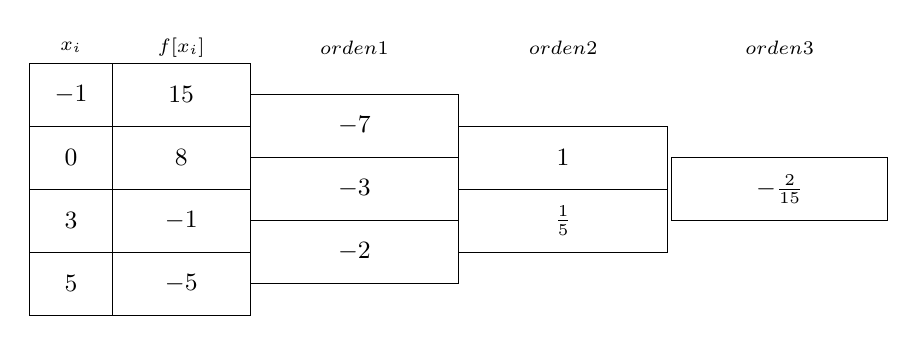
\begin{tikzpicture}[x=1cm,y=1cm]
\path[use as bounding box] (0,-3.65) rectangle (11,-0.0);
\node[font=\scriptsize] at (0.55,-0.25) {$x_i$};
\node[font=\scriptsize] at (1.95,-0.25) {$f[x_i]$};
\node[font=\scriptsize] at (4.15,-0.25) {$\text{orden }1$};
\node[font=\scriptsize] at (6.8,-0.25) {$\text{orden }2$};
\node[font=\scriptsize] at (9.55,-0.25) {$\text{orden }3$};
\node[draw,minimum width=1.05cm,minimum height=.8cm,inner sep=1pt,font=\small] at (0.55,-0.85) {$-1$};
\node[draw,minimum width=1.05cm,minimum height=.8cm,inner sep=1pt,font=\small] at (0.55,-1.65) {$0$};
\node[draw,minimum width=1.05cm,minimum height=.8cm,inner sep=1pt,font=\small] at (0.55,-2.45) {$3$};
\node[draw,minimum width=1.05cm,minimum height=.8cm,inner sep=1pt,font=\small] at (0.55,-3.2500000000000004) {$5$};
\node[draw,minimum width=1.75cm,minimum height=.8cm,inner sep=1pt,font=\small] at (1.95,-0.85) {$15$};
\node[draw,minimum width=1.75cm,minimum height=.8cm,inner sep=1pt,font=\small] at (1.95,-1.65) {$8$};
\node[draw,minimum width=1.75cm,minimum height=.8cm,inner sep=1pt,font=\small] at (1.95,-2.45) {$-1$};
\node[draw,minimum width=1.75cm,minimum height=.8cm,inner sep=1pt,font=\small] at (1.95,-3.2500000000000004) {$-5$};
\node[draw,minimum width=2.65cm,minimum height=.8cm,inner sep=1pt,font=\small] at (4.15,-1.25) {$-7$};
\node[draw,minimum width=2.65cm,minimum height=.8cm,inner sep=1pt,font=\small] at (4.15,-2.05) {$-3$};
\node[draw,minimum width=2.65cm,minimum height=.8cm,inner sep=1pt,font=\small] at (4.15,-2.85) {$-2$};
\node[draw,minimum width=2.65cm,minimum height=.8cm,inner sep=1pt,font=\small] at (6.8,-1.65) {$1$};
\node[draw,minimum width=2.65cm,minimum height=.8cm,inner sep=1pt,font=\small] at (6.8,-2.45) {$\frac15$};
\node[draw,minimum width=2.75cm,minimum height=.8cm,inner sep=1pt,font=\small] at (9.55,-2.0500000000000003) {$-\frac2{15}$};
\end{tikzpicture}\end{center}
\[f[-1,0,3,5]=\frac{1/5-1}{5-(-1)}=-\frac2{15}.\]
\end{frame}
\begin{frame}[t]{Diferencias divididas: ampliación}
\par\noindent\begin{minipage}[t][12mm][t]{\textwidth}\small\strut Ampliar el polinomio con el nuevo dato $x_3=5$, $f(5)=-5$.\end{minipage}\par\nointerlineskip
\begin{center}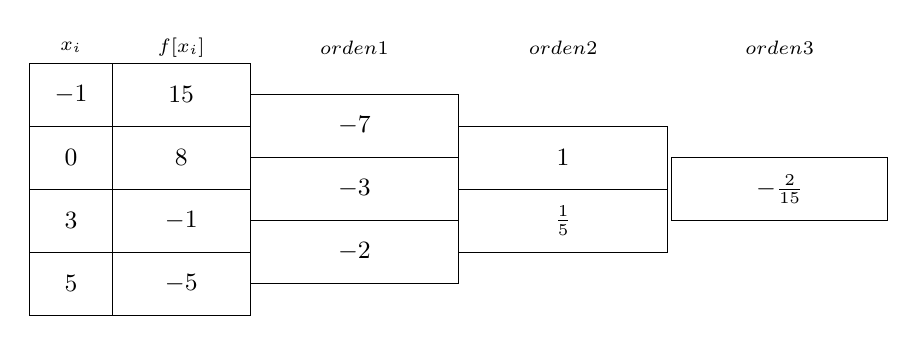
\begin{tikzpicture}[x=1cm,y=1cm]
\path[use as bounding box] (0,-3.65) rectangle (11,-0.0);
\node[font=\scriptsize] at (0.55,-0.25) {$x_i$};
\node[font=\scriptsize] at (1.95,-0.25) {$f[x_i]$};
\node[font=\scriptsize] at (4.15,-0.25) {$\text{orden }1$};
\node[font=\scriptsize] at (6.8,-0.25) {$\text{orden }2$};
\node[font=\scriptsize] at (9.55,-0.25) {$\text{orden }3$};
\node[draw,minimum width=1.05cm,minimum height=.8cm,inner sep=1pt,font=\small] at (0.55,-0.85) {$-1$};
\node[draw,minimum width=1.05cm,minimum height=.8cm,inner sep=1pt,font=\small] at (0.55,-1.65) {$0$};
\node[draw,minimum width=1.05cm,minimum height=.8cm,inner sep=1pt,font=\small] at (0.55,-2.45) {$3$};
\node[draw,minimum width=1.05cm,minimum height=.8cm,inner sep=1pt,font=\small] at (0.55,-3.2500000000000004) {$5$};
\node[draw,minimum width=1.75cm,minimum height=.8cm,inner sep=1pt,font=\small] at (1.95,-0.85) {$15$};
\node[draw,minimum width=1.75cm,minimum height=.8cm,inner sep=1pt,font=\small] at (1.95,-1.65) {$8$};
\node[draw,minimum width=1.75cm,minimum height=.8cm,inner sep=1pt,font=\small] at (1.95,-2.45) {$-1$};
\node[draw,minimum width=1.75cm,minimum height=.8cm,inner sep=1pt,font=\small] at (1.95,-3.2500000000000004) {$-5$};
\node[draw,minimum width=2.65cm,minimum height=.8cm,inner sep=1pt,font=\small] at (4.15,-1.25) {$-7$};
\node[draw,minimum width=2.65cm,minimum height=.8cm,inner sep=1pt,font=\small] at (4.15,-2.05) {$-3$};
\node[draw,minimum width=2.65cm,minimum height=.8cm,inner sep=1pt,font=\small] at (4.15,-2.85) {$-2$};
\node[draw,minimum width=2.65cm,minimum height=.8cm,inner sep=1pt,font=\small] at (6.8,-1.65) {$1$};
\node[draw,minimum width=2.65cm,minimum height=.8cm,inner sep=1pt,font=\small] at (6.8,-2.45) {$\frac15$};
\node[draw,minimum width=2.75cm,minimum height=.8cm,inner sep=1pt,font=\small] at (9.55,-2.0500000000000003) {$-\frac2{15}$};
\end{tikzpicture}\end{center}
\small\[P_3(x)=P_2(x)-\frac2{15}(x+1)x(x-3).\]
\end{frame}
\begin{frame}[t]{Diferencias divididas: ampliación}
\par\noindent\begin{minipage}[t][12mm][t]{\textwidth}\small\strut Ampliar el polinomio con el nuevo dato $x_3=5$, $f(5)=-5$.\end{minipage}\par\nointerlineskip
\begin{center}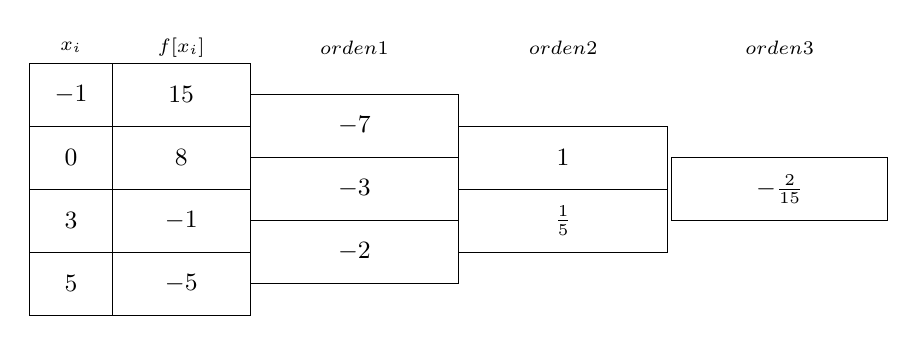
\begin{tikzpicture}[x=1cm,y=1cm]
\path[use as bounding box] (0,-3.65) rectangle (11,-0.0);
\node[font=\scriptsize] at (0.55,-0.25) {$x_i$};
\node[font=\scriptsize] at (1.95,-0.25) {$f[x_i]$};
\node[font=\scriptsize] at (4.15,-0.25) {$\text{orden }1$};
\node[font=\scriptsize] at (6.8,-0.25) {$\text{orden }2$};
\node[font=\scriptsize] at (9.55,-0.25) {$\text{orden }3$};
\node[draw,minimum width=1.05cm,minimum height=.8cm,inner sep=1pt,font=\small] at (0.55,-0.85) {$-1$};
\node[draw,minimum width=1.05cm,minimum height=.8cm,inner sep=1pt,font=\small] at (0.55,-1.65) {$0$};
\node[draw,minimum width=1.05cm,minimum height=.8cm,inner sep=1pt,font=\small] at (0.55,-2.45) {$3$};
\node[draw,minimum width=1.05cm,minimum height=.8cm,inner sep=1pt,font=\small] at (0.55,-3.2500000000000004) {$5$};
\node[draw,minimum width=1.75cm,minimum height=.8cm,inner sep=1pt,font=\small] at (1.95,-0.85) {$15$};
\node[draw,minimum width=1.75cm,minimum height=.8cm,inner sep=1pt,font=\small] at (1.95,-1.65) {$8$};
\node[draw,minimum width=1.75cm,minimum height=.8cm,inner sep=1pt,font=\small] at (1.95,-2.45) {$-1$};
\node[draw,minimum width=1.75cm,minimum height=.8cm,inner sep=1pt,font=\small] at (1.95,-3.2500000000000004) {$-5$};
\node[draw,minimum width=2.65cm,minimum height=.8cm,inner sep=1pt,font=\small] at (4.15,-1.25) {$-7$};
\node[draw,minimum width=2.65cm,minimum height=.8cm,inner sep=1pt,font=\small] at (4.15,-2.05) {$-3$};
\node[draw,minimum width=2.65cm,minimum height=.8cm,inner sep=1pt,font=\small] at (4.15,-2.85) {$-2$};
\node[draw,minimum width=2.65cm,minimum height=.8cm,inner sep=1pt,font=\small] at (6.8,-1.65) {$1$};
\node[draw,minimum width=2.65cm,minimum height=.8cm,inner sep=1pt,font=\small] at (6.8,-2.45) {$\frac15$};
\node[draw,minimum width=2.75cm,minimum height=.8cm,inner sep=1pt,font=\small] at (9.55,-2.0500000000000003) {$-\frac2{15}$};
\end{tikzpicture}\end{center}
\small\[P_3(x)=-\frac2{15}x^3+\frac{19}{15}x^2-\frac{28}{5}x+8.\]
\end{frame}
\end{document}
